% Preamble
\documentclass{article}

\usepackage[a4paper, left=2.5cm, right=2cm, top=3cm, bottom=3cm]{geometry}
\usepackage{graphicx}
\usepackage{cite}
\usepackage{amssymb}
\usepackage{amsmath}
\usepackage{ulem}
\usepackage{subcaption}
\usepackage{caption}
\usepackage{float}
\usepackage{hyperref}
\usepackage{placeins}

% Title
\title{Introduction to Machine Learning: Work 3}
\author{
	Pedro Agúndez\textsuperscript{*}, 
	Bruno Sánchez\textsuperscript{*}, 
	María del Carmen Ramírez\textsuperscript{*}, 
	Antonio Lobo\textsuperscript{*}
}
\date{December 8, 2024}

% Document
\begin{document}

\maketitle
\renewcommand{\thefootnote}{\fnsymbol{footnote}}
\footnotetext[1]{Universitat de Barcelona \\ 
    \texttt{pedro.agundez@estudiantat.upc.edu} \\
    \texttt{bruno.sanchez.gomez@estudiantat.upc.edu} \\
    \texttt{maria.del.carmen.ramirez@estudiantat.upc.edu} \\
    \texttt{antonio.lobo@estudiantat.upc.edu}
}

\begin{abstract}
We investigate the clustering performance of \textbf{K-Means}, \textbf{Global K-Means}, \textbf{X-Means}, \textbf{Fuzzy C-Means (FCM)}, and \textbf{Spectral Clustering} across three datasets: \textbf{Hepatitis}, \textbf{Mushroom}, and \textbf{Pen-based}. Each algorithm is assessed with various hyperparameters, distance metrics (\textbf{Euclidean}, \textbf{Manhattan}, \textbf{Clark}), and cluster validity indices (\textbf{ARI}, \textbf{NMI}, \textbf{DBI}, \textbf{Silhouette}, \textbf{CHS}). Dimensionality reduction techniques (\textbf{PCA}, \textbf{UMAP}) support visualization and interpretation. Our results show that \textbf{Global K-Means} improves consistency over standard \textbf{K-Means}, while \textbf{FCM} demonstrates flexibility with datasets of differing density and structure. These findings highlight the importance of algorithmic configuration and data characteristics in achieving robust clustering performance. 
\end{abstract}

\newpage

\section{Introduction}
\textbf{Clustering algorithms} aim to uncover natural groupings in unlabeled data, but their \textbf{effectiveness} depends on the \textbf{choice of algorithm}, \textbf{hyperparameters}, and \textbf{data characteristics}. This work systematically compares \textbf{K-Means}, its \textbf{variations Global K-Means and X-Means}, \textbf{Optics} (a \textbf{density-based ordering method}), \textbf{Spectral Clustering} (a \textbf{graph-based partitioning method}), and \textbf{Fuzzy C-Means (FCM)} (based on \textbf{fuzzy sets}) on three diverse datasets: \textbf{Hepatitis}, \textbf{Mushroom}, and \textbf{Pen-based}.

We evaluate clustering performance using multiple metrics, including \textbf{ARI}, \textbf{NMI}, \textbf{DBI}, \textbf{Silhouette}, and \textbf{CHS scores}. Dimensionality reduction methods, such as \textbf{PCA} and \textbf{UMAP}, are applied to visualize high-dimensional datasets effectively.

Our analysis identifies key trends in algorithm behavior, such as the \textbf{stability of Global K-Means}, the \textbf{adaptability of FCM} to varying densities, the \textbf{flexibility of X-Means} in determining the number of clusters, and the \textbf{sensitivity of Optics and Spectral Clustering} to complex data structures. These insights guide the \textbf{selection of clustering methods} tailored to specific datasets and objectives.
\section{Methodology}
Introduction to methodology.

\subsection{K-Means}
We have tested on each dataset 57 different configurations of the K-Means algorithm, by using the 3 different distance metrics with 19 different values of the k (from 2 to 20). For each of these configurations, we have run the K-Means 10 times, in order to account for the randomness of the centroid initialization. This results in a total of 570 runs of the K-Means algorithm for each dataset. From the evaluation metrics extracted for each of these runs, we study the effect of each of the 2 hyperparameters and achieve conclusions about them through statistical analysis.

\subsubsection{Preliminary Study}
Before starting with the more rigorous statistical analysis, let us first observe some preliminary patterns about the measured metrics and the effect of each hyperparameter on the clustering performance.

In Figure \ref{fig:metrics_corr} we summarize the relationship between the different metrics that were measured. It is a matrix plot where the lower triangle is a heatmap of the Pearson correlations between each pair of metrics, the diagonal elements are the histogram distributions of values of each metric, and the upper triangular has for each pair of metrics the plot of their values for all runs. It is interesting to observe that, while we would expect all of the metrics to agree on the identified trends, there are some cases where the opposite behaviour is displayed. An example of this is the negative correlation between E (total variance) and DBI (Davies-Bouldin Index): since the DBI measures cluster compactness, we would expect it to directly correlate to E; however, we observe that there is a negative correlation between them. This specific figure was extracted from the results on the Mushroom dataset, but the conclusions are the same for the others (the plots can be found in the \texttt{code} floder).

\begin{figure}[h]
    \centering
    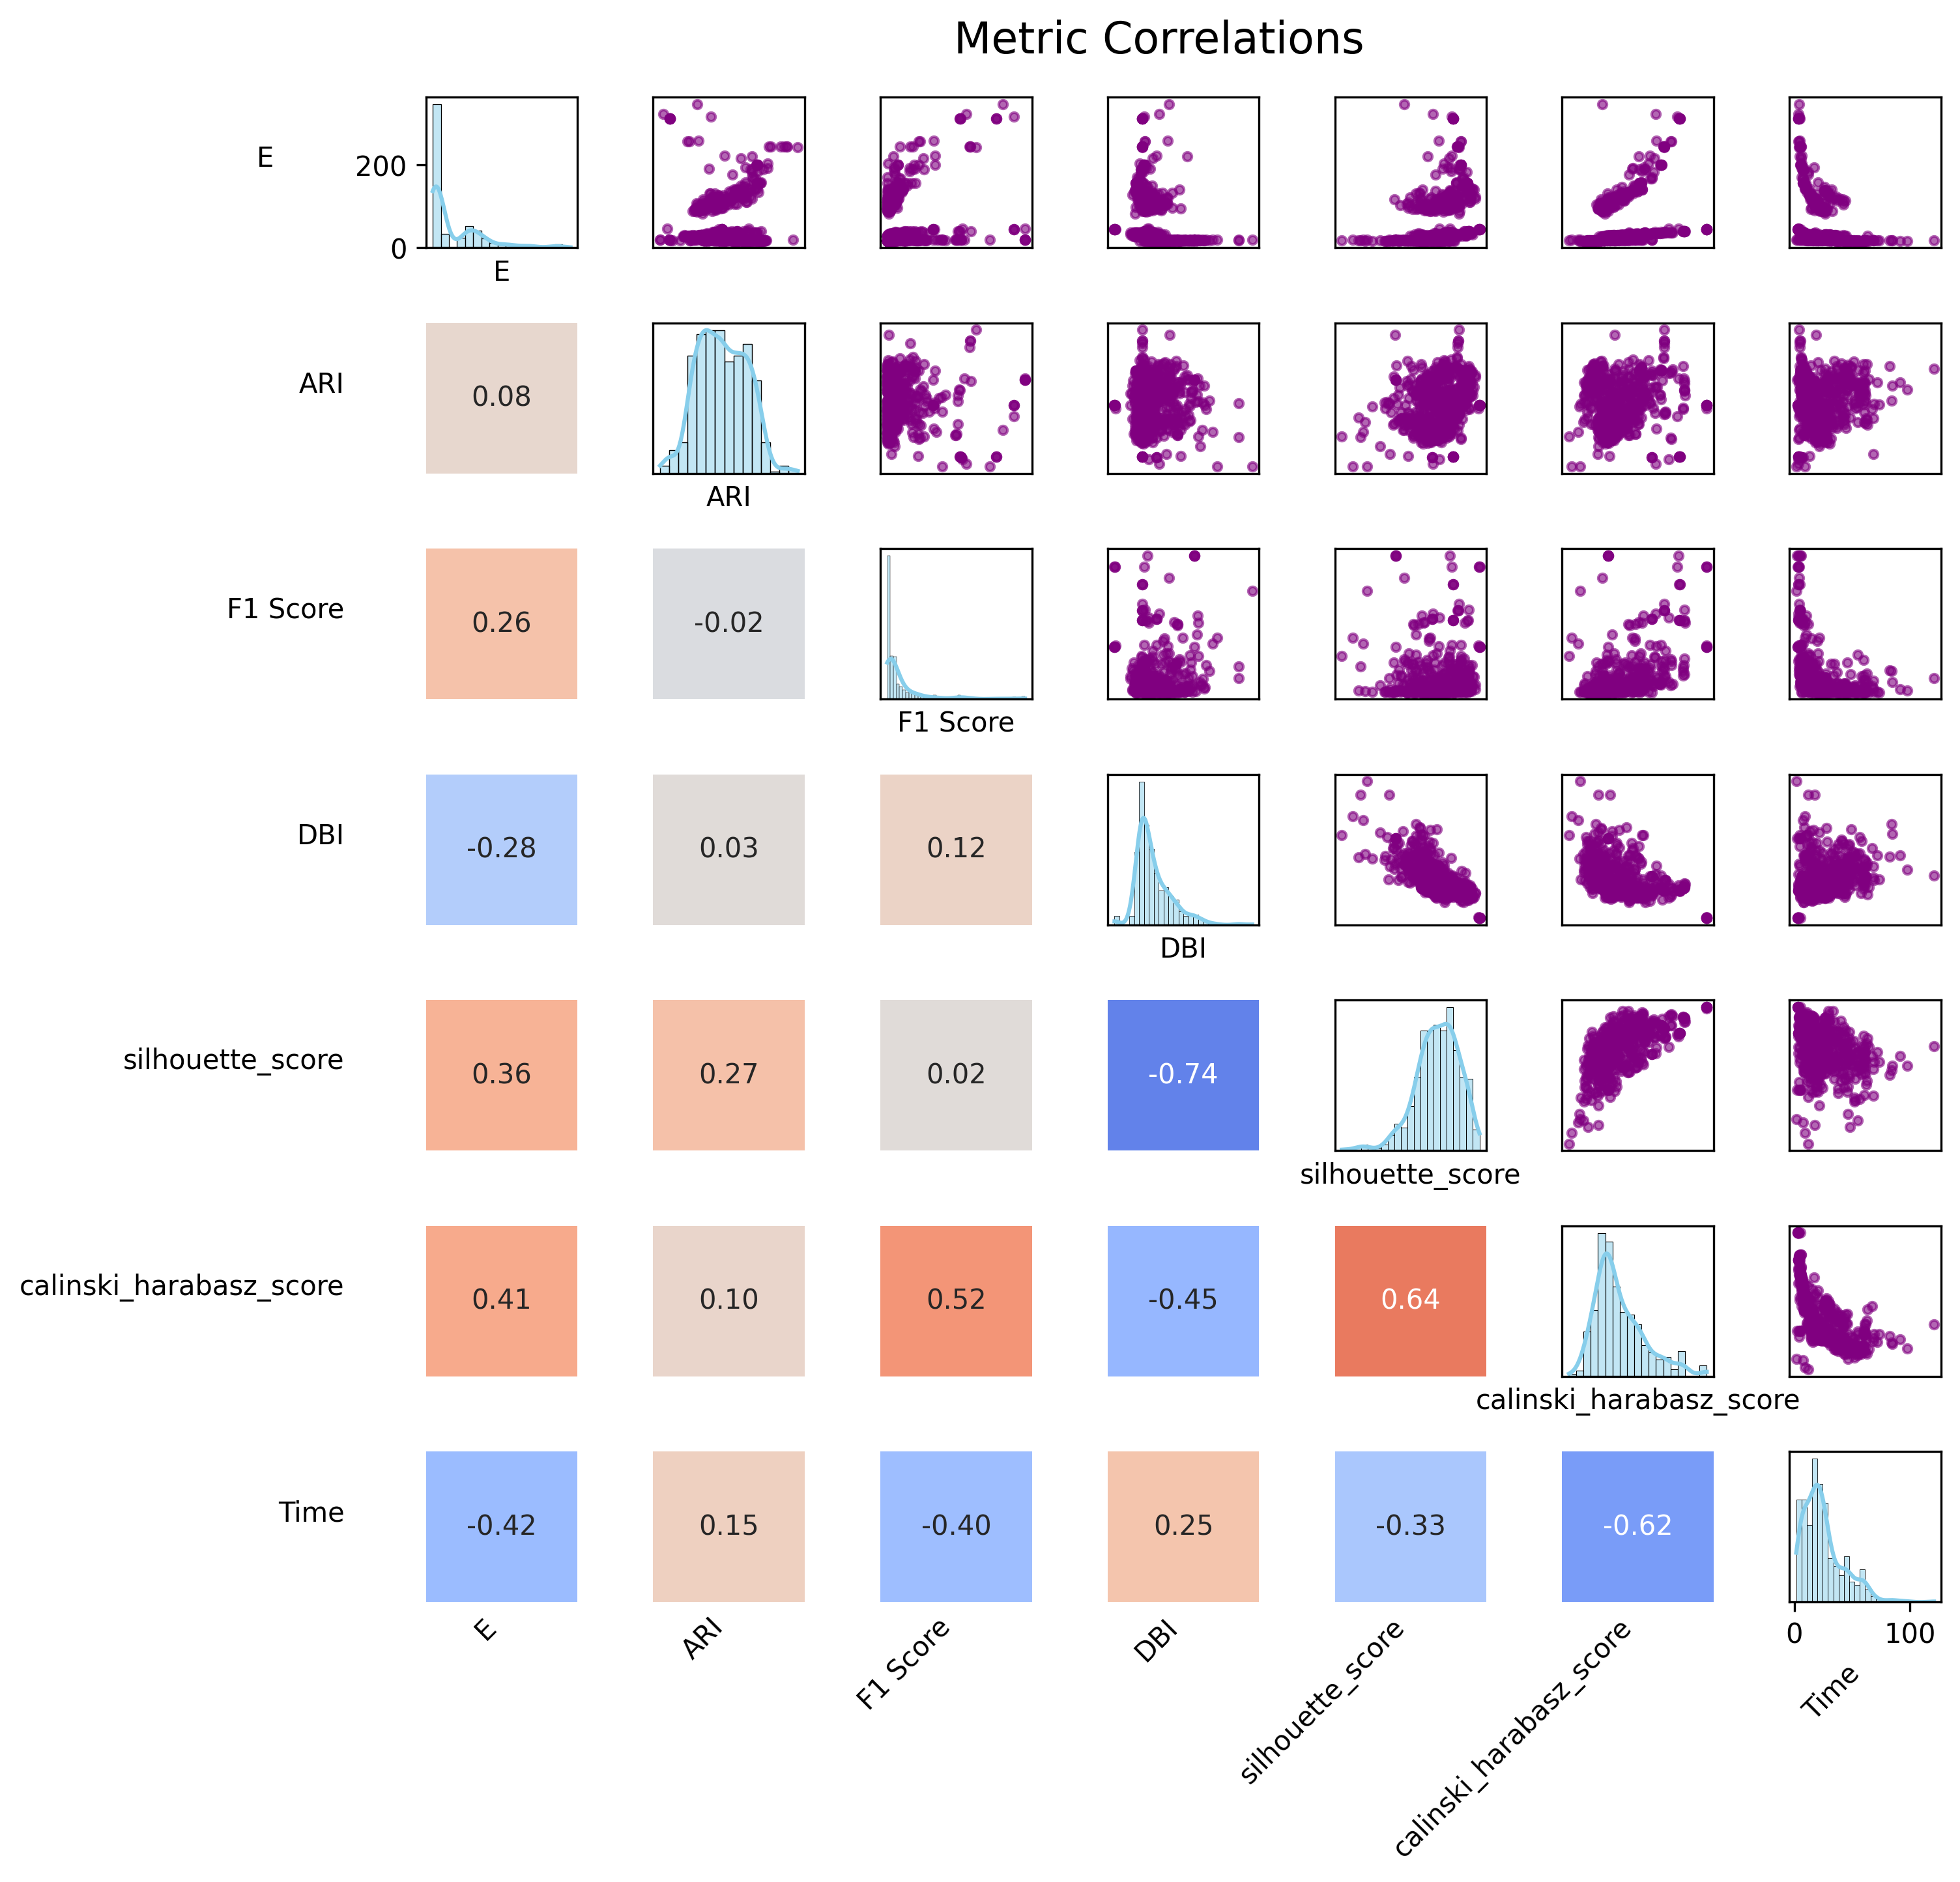
\includegraphics[width=0.7\textwidth]{figures/metrics_correlations_matrix.png}
    \caption{Metrics correlations summary}
    \label{fig:metrics_corr}
\end{figure}

Parallelly, a different set of interesting relationship are displayed in Figure \ref{fig:pairplot}, where we can see heatmaps of the F1 Score and the Time across the different pairwise hyperparameter configurations. We can observe a general trend regarding execution time: it seems to have considerably larger values for the Clark distance metric compared to those of the other 2, which reflects the higher computational cost that this distance metric has. Additionally, we see a noteworthy divergence in the F1 Score trends with respect to the values of k: in the Mushroom dataset (which has 2 classes), lower values of k seem to achieve a better F1 Score; meanwhile, in the Pen-based dataset (which has 10 classes), intermediate values of k (between 7 and 11) seem to achieve the best scores. This was to be expected, yet it still is compelling to see it reflected so clearly in the results. 

\begin{figure}[H]
    \centering
    \begin{subfigure}{0.49\textwidth}
        \centering
        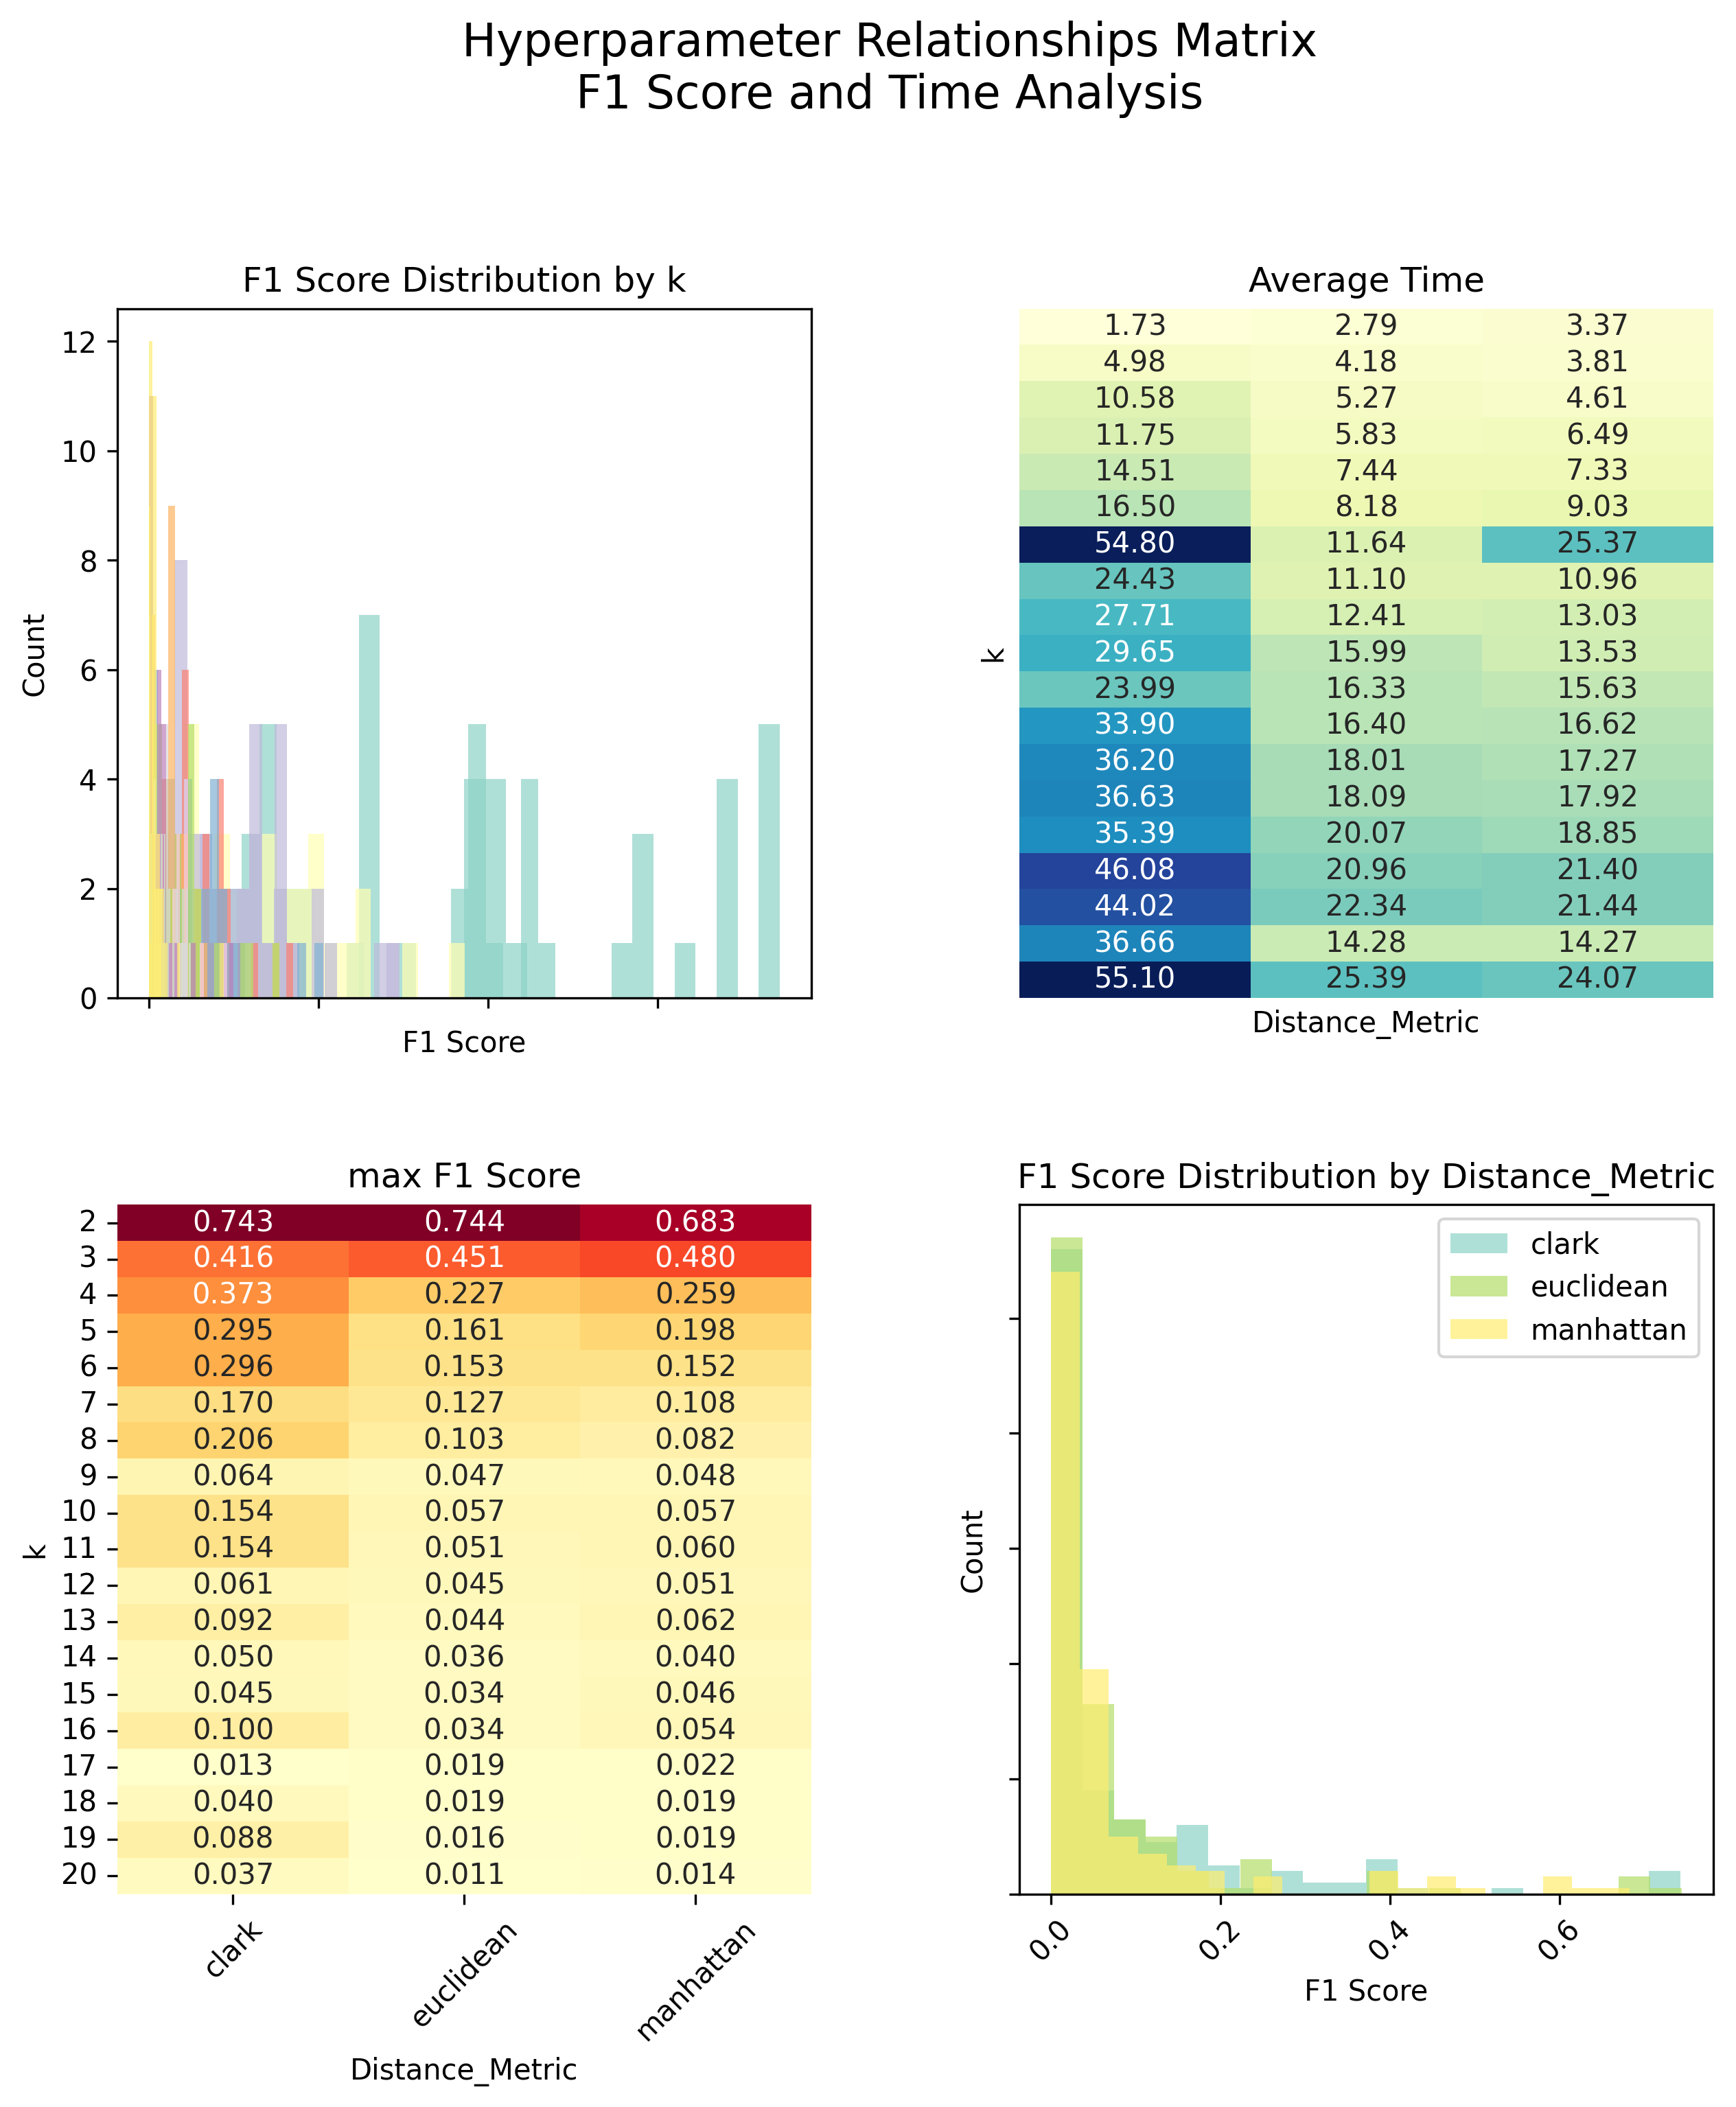
\includegraphics[width=\linewidth]{figures/mushroom_hyperparameter_pairplot_matrix.png}
        \caption{Mushroom pairplot matrix}
    \end{subfigure}
    \hfill
    \begin{subfigure}{0.49\textwidth}
        \centering
        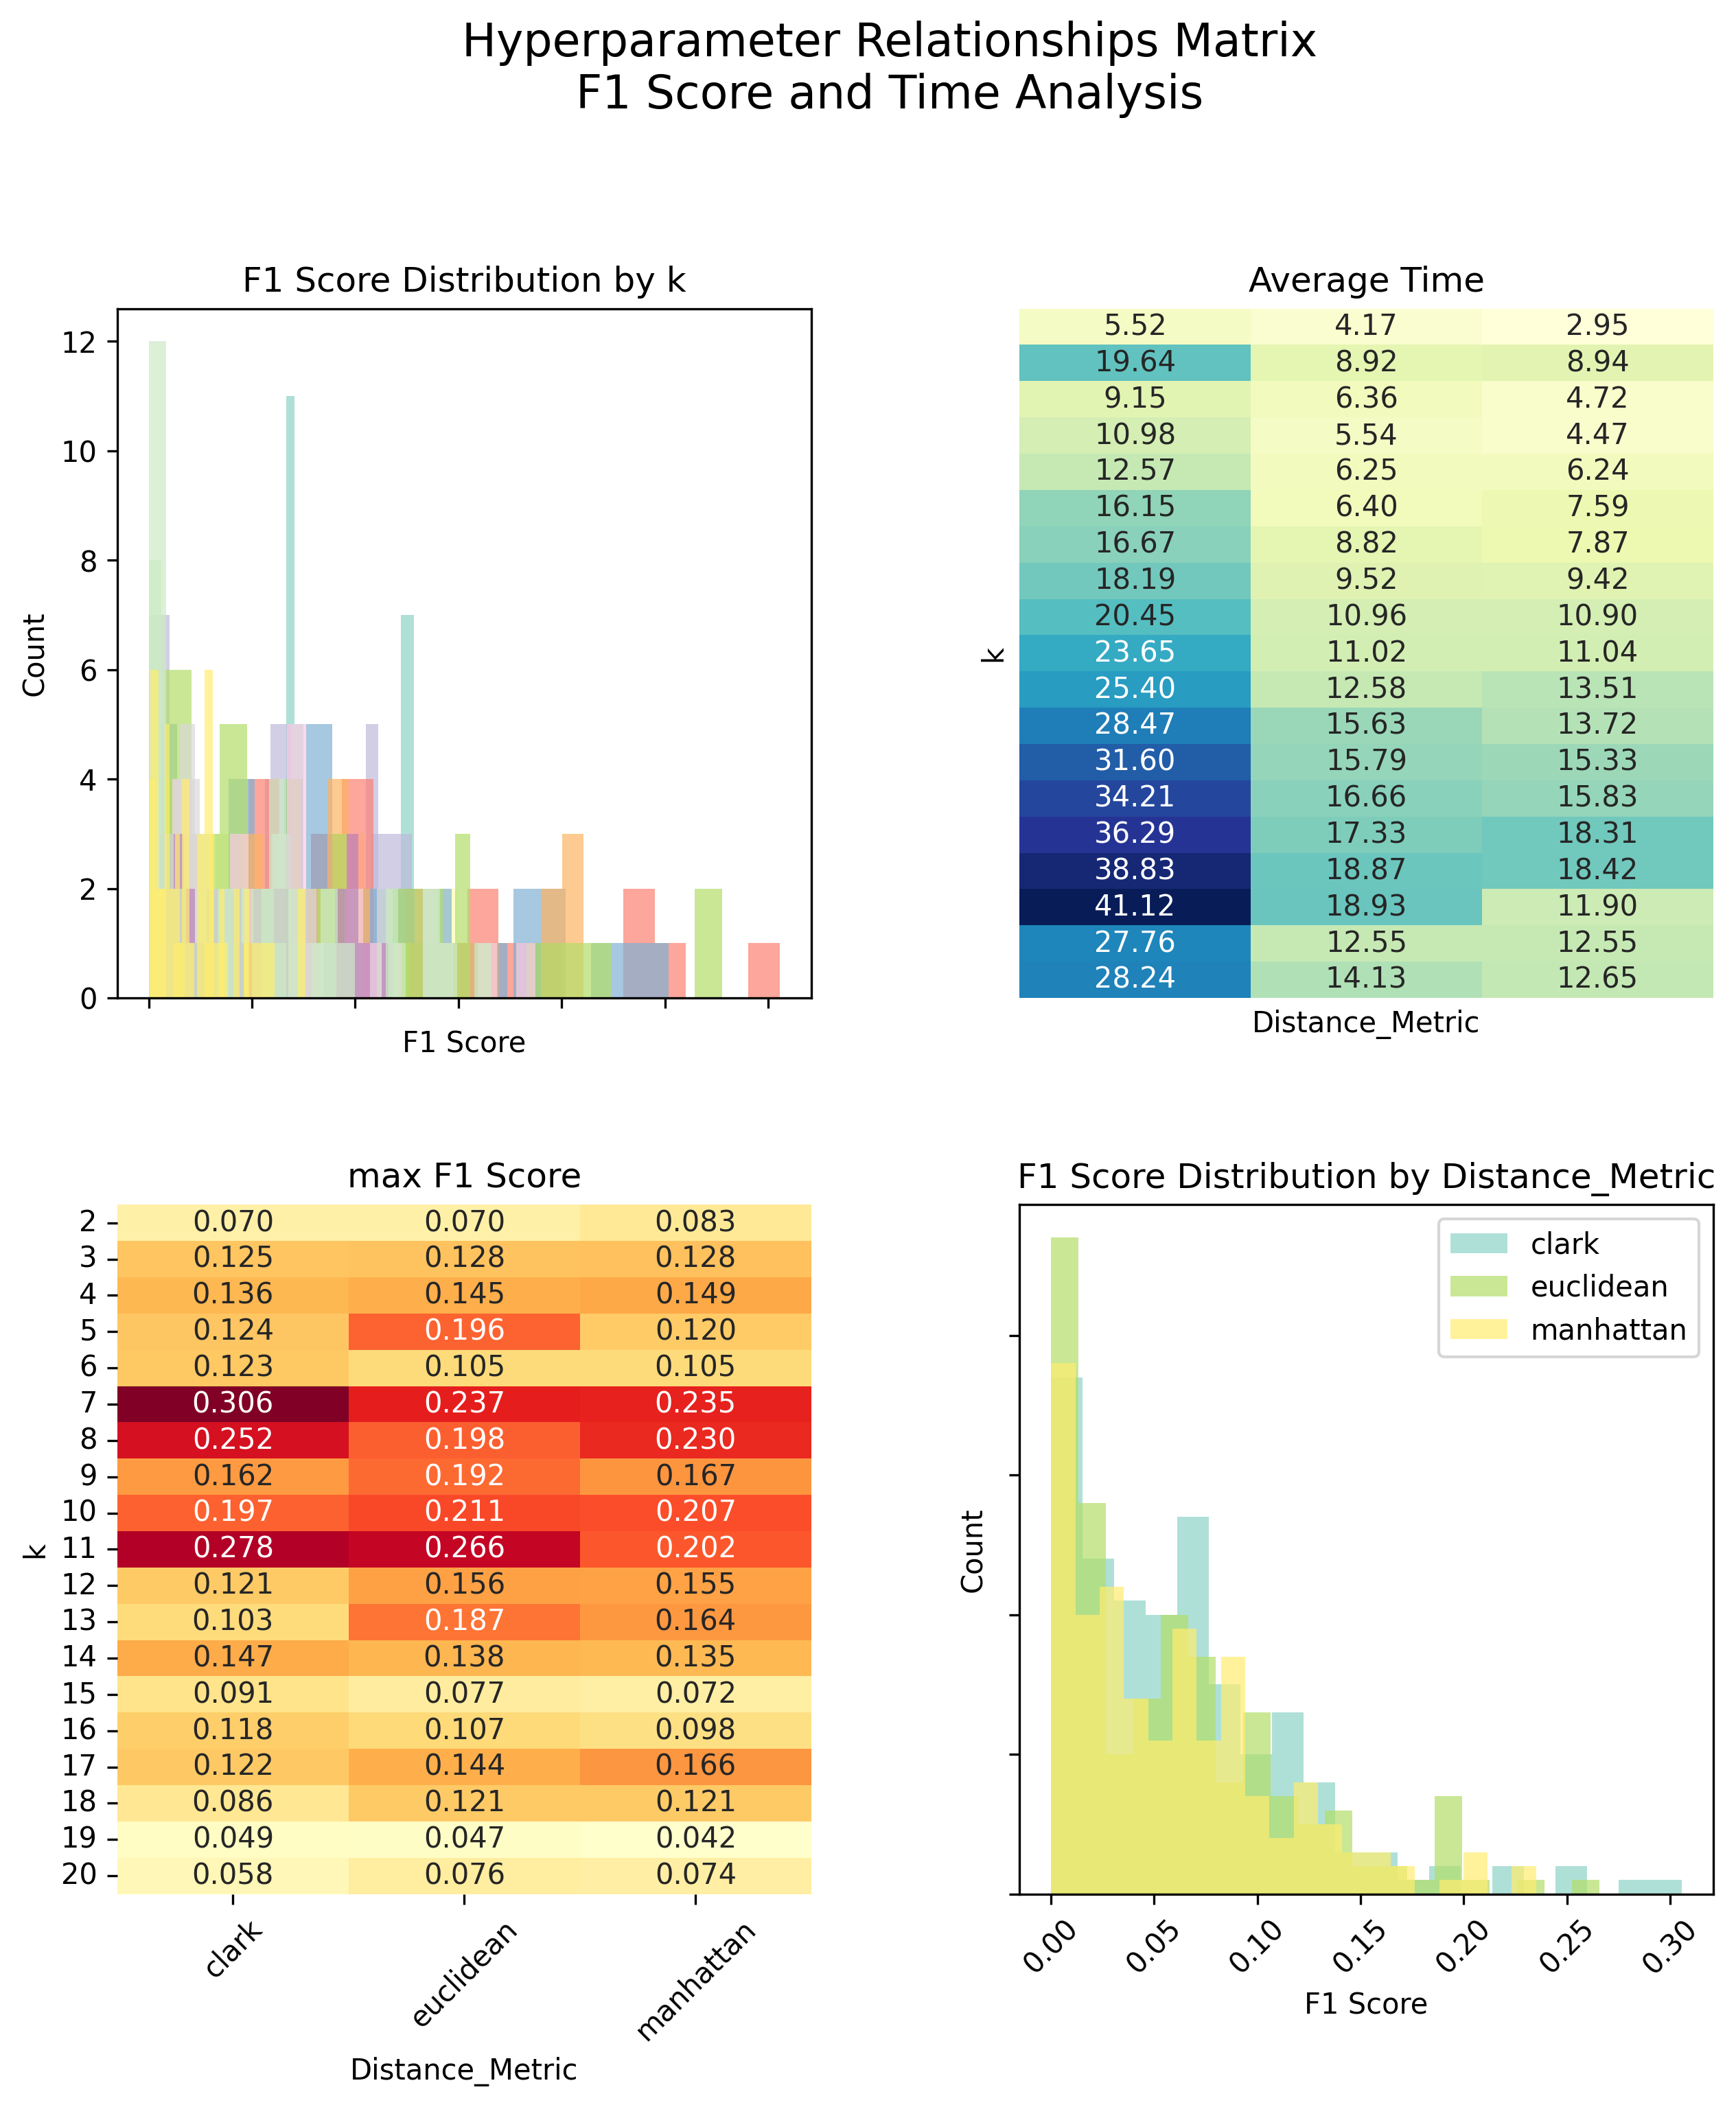
\includegraphics[width=\linewidth]{figures/penbased_hyperparameter_pairplot_matrix.png}
        \caption{Pen-based pairplot matrix}
    \end{subfigure}
    \caption{Hyperparameter pairplot matrices based on F1 Score and Time}
    \label{fig:pairplot}
\end{figure}

\subsubsection{Statistical Analysis}
For the statistical analysis, we have first performed Friedman tests to determine if there are significant differences in each of the metrics for the different possible values of each hyperparameter. 

\subsection{Fuzzy C-Means}
\section{Results}\label{sec:results}
To systematically evaluate the different configurations of each clustering algorithm, the following procedure is followed to extract results for each of the 3 data sets, in order to later perform an analysis those results:

\begin{enumerate}
    \item \textbf{Data Preparation}: The dataset is loaded and the data samples are separated from their labels into separate 2 sets. This way, we perform the clustering analysis in a completely non-supervised way, and we then utilize the labels to extract supervised metrics of the cultering results.

    \item \textbf{Parameter Configuration}: A comprehensive set of values for the algorithm's hyperparameters is defined. These combinations reflect various ways to tune the clustering algorithm.

    \item \textbf{Model Evaluation}: For each parameter combination, the clustering algorithm is applied on the unlabeled data and then evaluated with different metrics. This step yields the following metrics: Adjusted Rand Score (ARI), Normalized Mutual Information (NMI), Davies-Bouldin Index(DBI), Silhouette score, Calinski-Harabasz Score (CHS), and execution time. Together, these metrics (the first 2 supervised, and the rest non-supervised) measure the effectiveness and efficiency of the clustering.

    \item \textbf{Results Compilation}: The performance metrics for each parameter combination are recorded in a structured format. These results are saved as a dataset that summarizes the outcomes of all evaluations, forming a basis for analysis. We save as well the cluster labels of all samples for each clustering algorithm that we run, so we can recover the same clusters in the posterior analysis.

    \item \textbf{Results Analysis}: After results are compiled across all configurations, quantitative and qualitative analysis is performed to identify common trends among the different algorithm configurations for each of the datasets. Additionally, we extract the top performing configuration according to each of the 5 evaluation metrics, in order to study common patterns and visualize the resulting clusters. This analysis helps determine the most reliable and effective parameter settings for accurate and efficient clustering for each dataset.
\end{enumerate}
Due to the vast ammount of information that can be extracted from the results, we will only explicitly showcase the most clarifying plots and results that we have extracted. However, all of the information is available in the \texttt{plots\_and\_tables} folder for each of the datasets, in the \texttt{code} attached to this report.

\textit{Note:} Since all of the tested datasets have high dimensionality, we use Principal Component Analysis (PCA) to extract the 2 principal components in order to generate the clustering scatter plots of the datasets for visualization purposes.

\subsection{K-Means}
We have tested on each dataset 57 different configurations of the K-Means algorithm, by using the 3 different distance metrics with 19 different values of the k (from 2 to 20). For each of these configurations, we have run the K-Means 10 times, in order to account for the randomness of the centroid initialization. This results in a total of 570 runs of the K-Means algorithm for each dataset. From the evaluation metrics extracted for each of these runs, we study the effect of each of the 2 hyperparameters and achieve conclusions about them through statistical analysis.

\subsubsection{Preliminary Study}
Before starting with the more rigorous statistical analysis, let us first observe some preliminary patterns about the measured metrics and the effect of each hyperparameter on the clustering performance.

In Figure \ref{fig:metrics_corr} we summarize the relationship between the different metrics that were measured. It is a matrix plot where the lower triangle is a heatmap of the Pearson correlations between each pair of metrics, the diagonal elements are the histogram distributions of values of each metric, and the upper triangular has for each pair of metrics the plot of their values for all runs. It is interesting to observe that, while we would expect all of the metrics to agree on the identified trends, there are some cases where the opposite behaviour is displayed. An example of this is the negative correlation between E (total variance) and DBI (Davies-Bouldin Index): since the DBI measures cluster compactness, we would expect it to directly correlate to E; however, we observe that there is a negative correlation between them. This specific figure was extracted from the results on the Mushroom dataset, but the conclusions are the same for the others (the plots can be found in the \texttt{code} floder).

\begin{figure}[h]
    \centering
    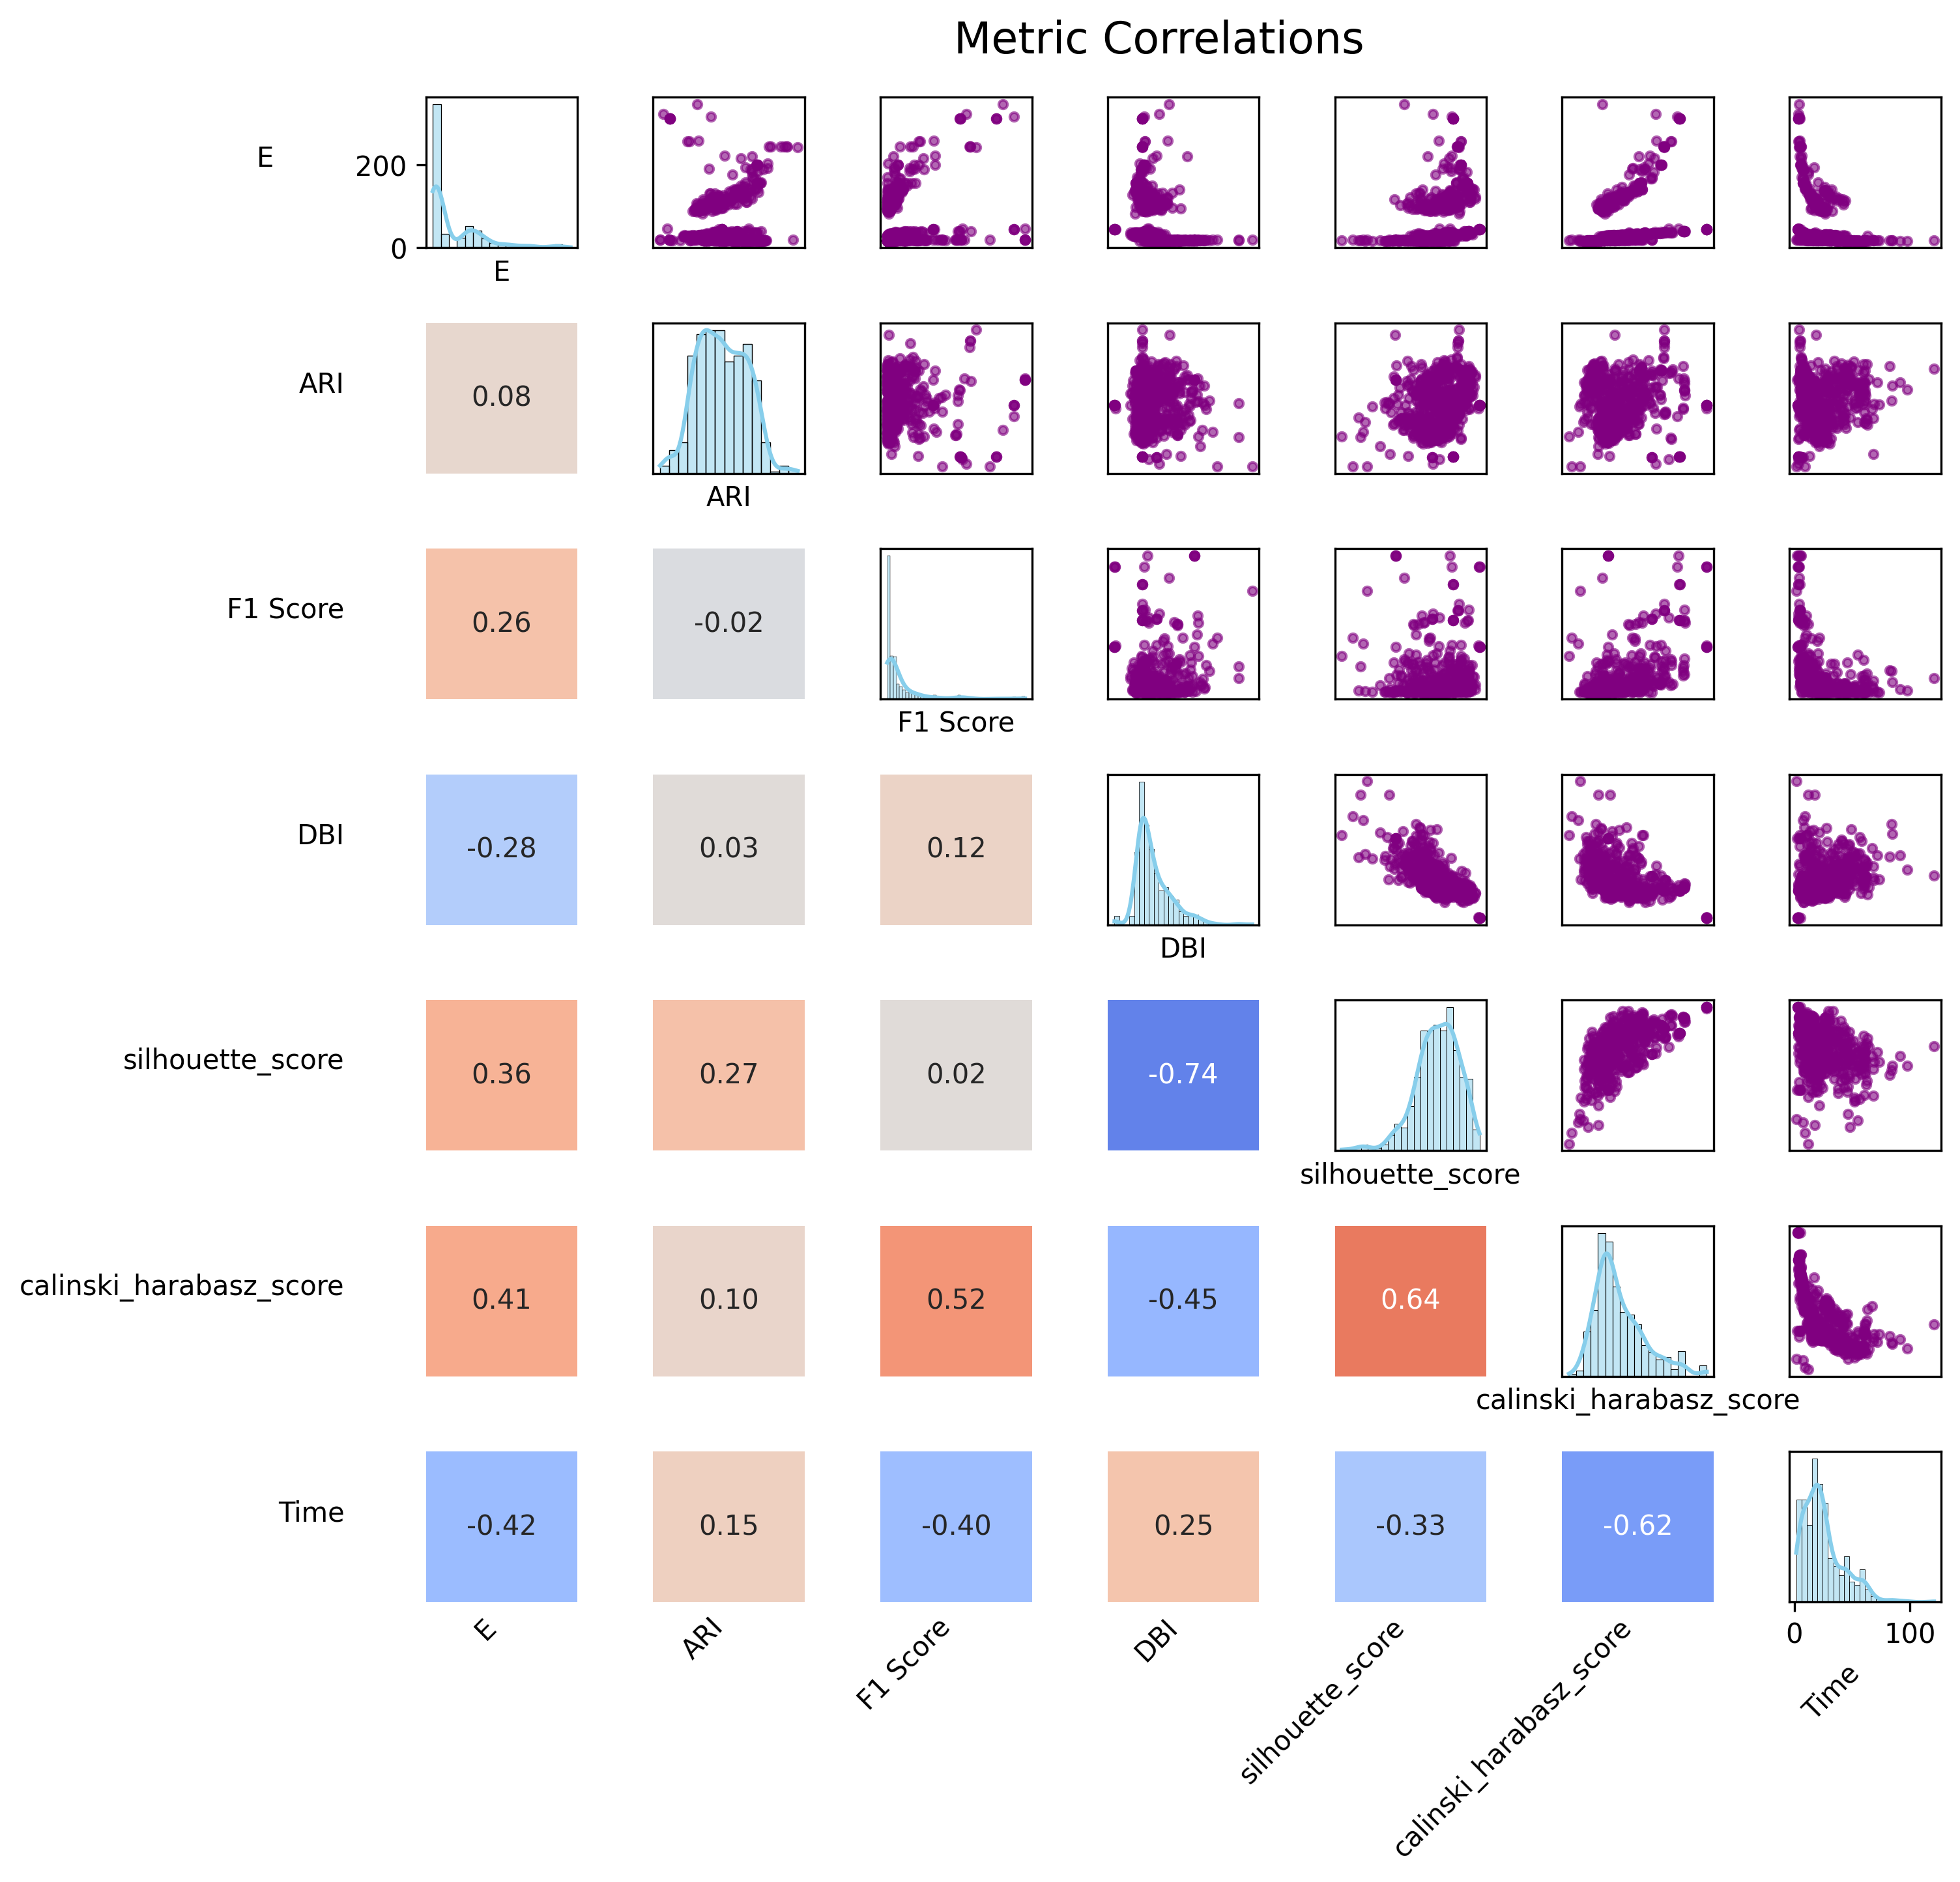
\includegraphics[width=0.7\textwidth]{figures/metrics_correlations_matrix.png}
    \caption{Metrics correlations summary}
    \label{fig:metrics_corr}
\end{figure}

Parallelly, a different set of interesting relationship are displayed in Figure \ref{fig:pairplot}, where we can see heatmaps of the F1 Score and the Time across the different pairwise hyperparameter configurations. We can observe a general trend regarding execution time: it seems to have considerably larger values for the Clark distance metric compared to those of the other 2, which reflects the higher computational cost that this distance metric has. Additionally, we see a noteworthy divergence in the F1 Score trends with respect to the values of k: in the Mushroom dataset (which has 2 classes), lower values of k seem to achieve a better F1 Score; meanwhile, in the Pen-based dataset (which has 10 classes), intermediate values of k (between 7 and 11) seem to achieve the best scores. This was to be expected, yet it still is compelling to see it reflected so clearly in the results. 

\begin{figure}[H]
    \centering
    \begin{subfigure}{0.49\textwidth}
        \centering
        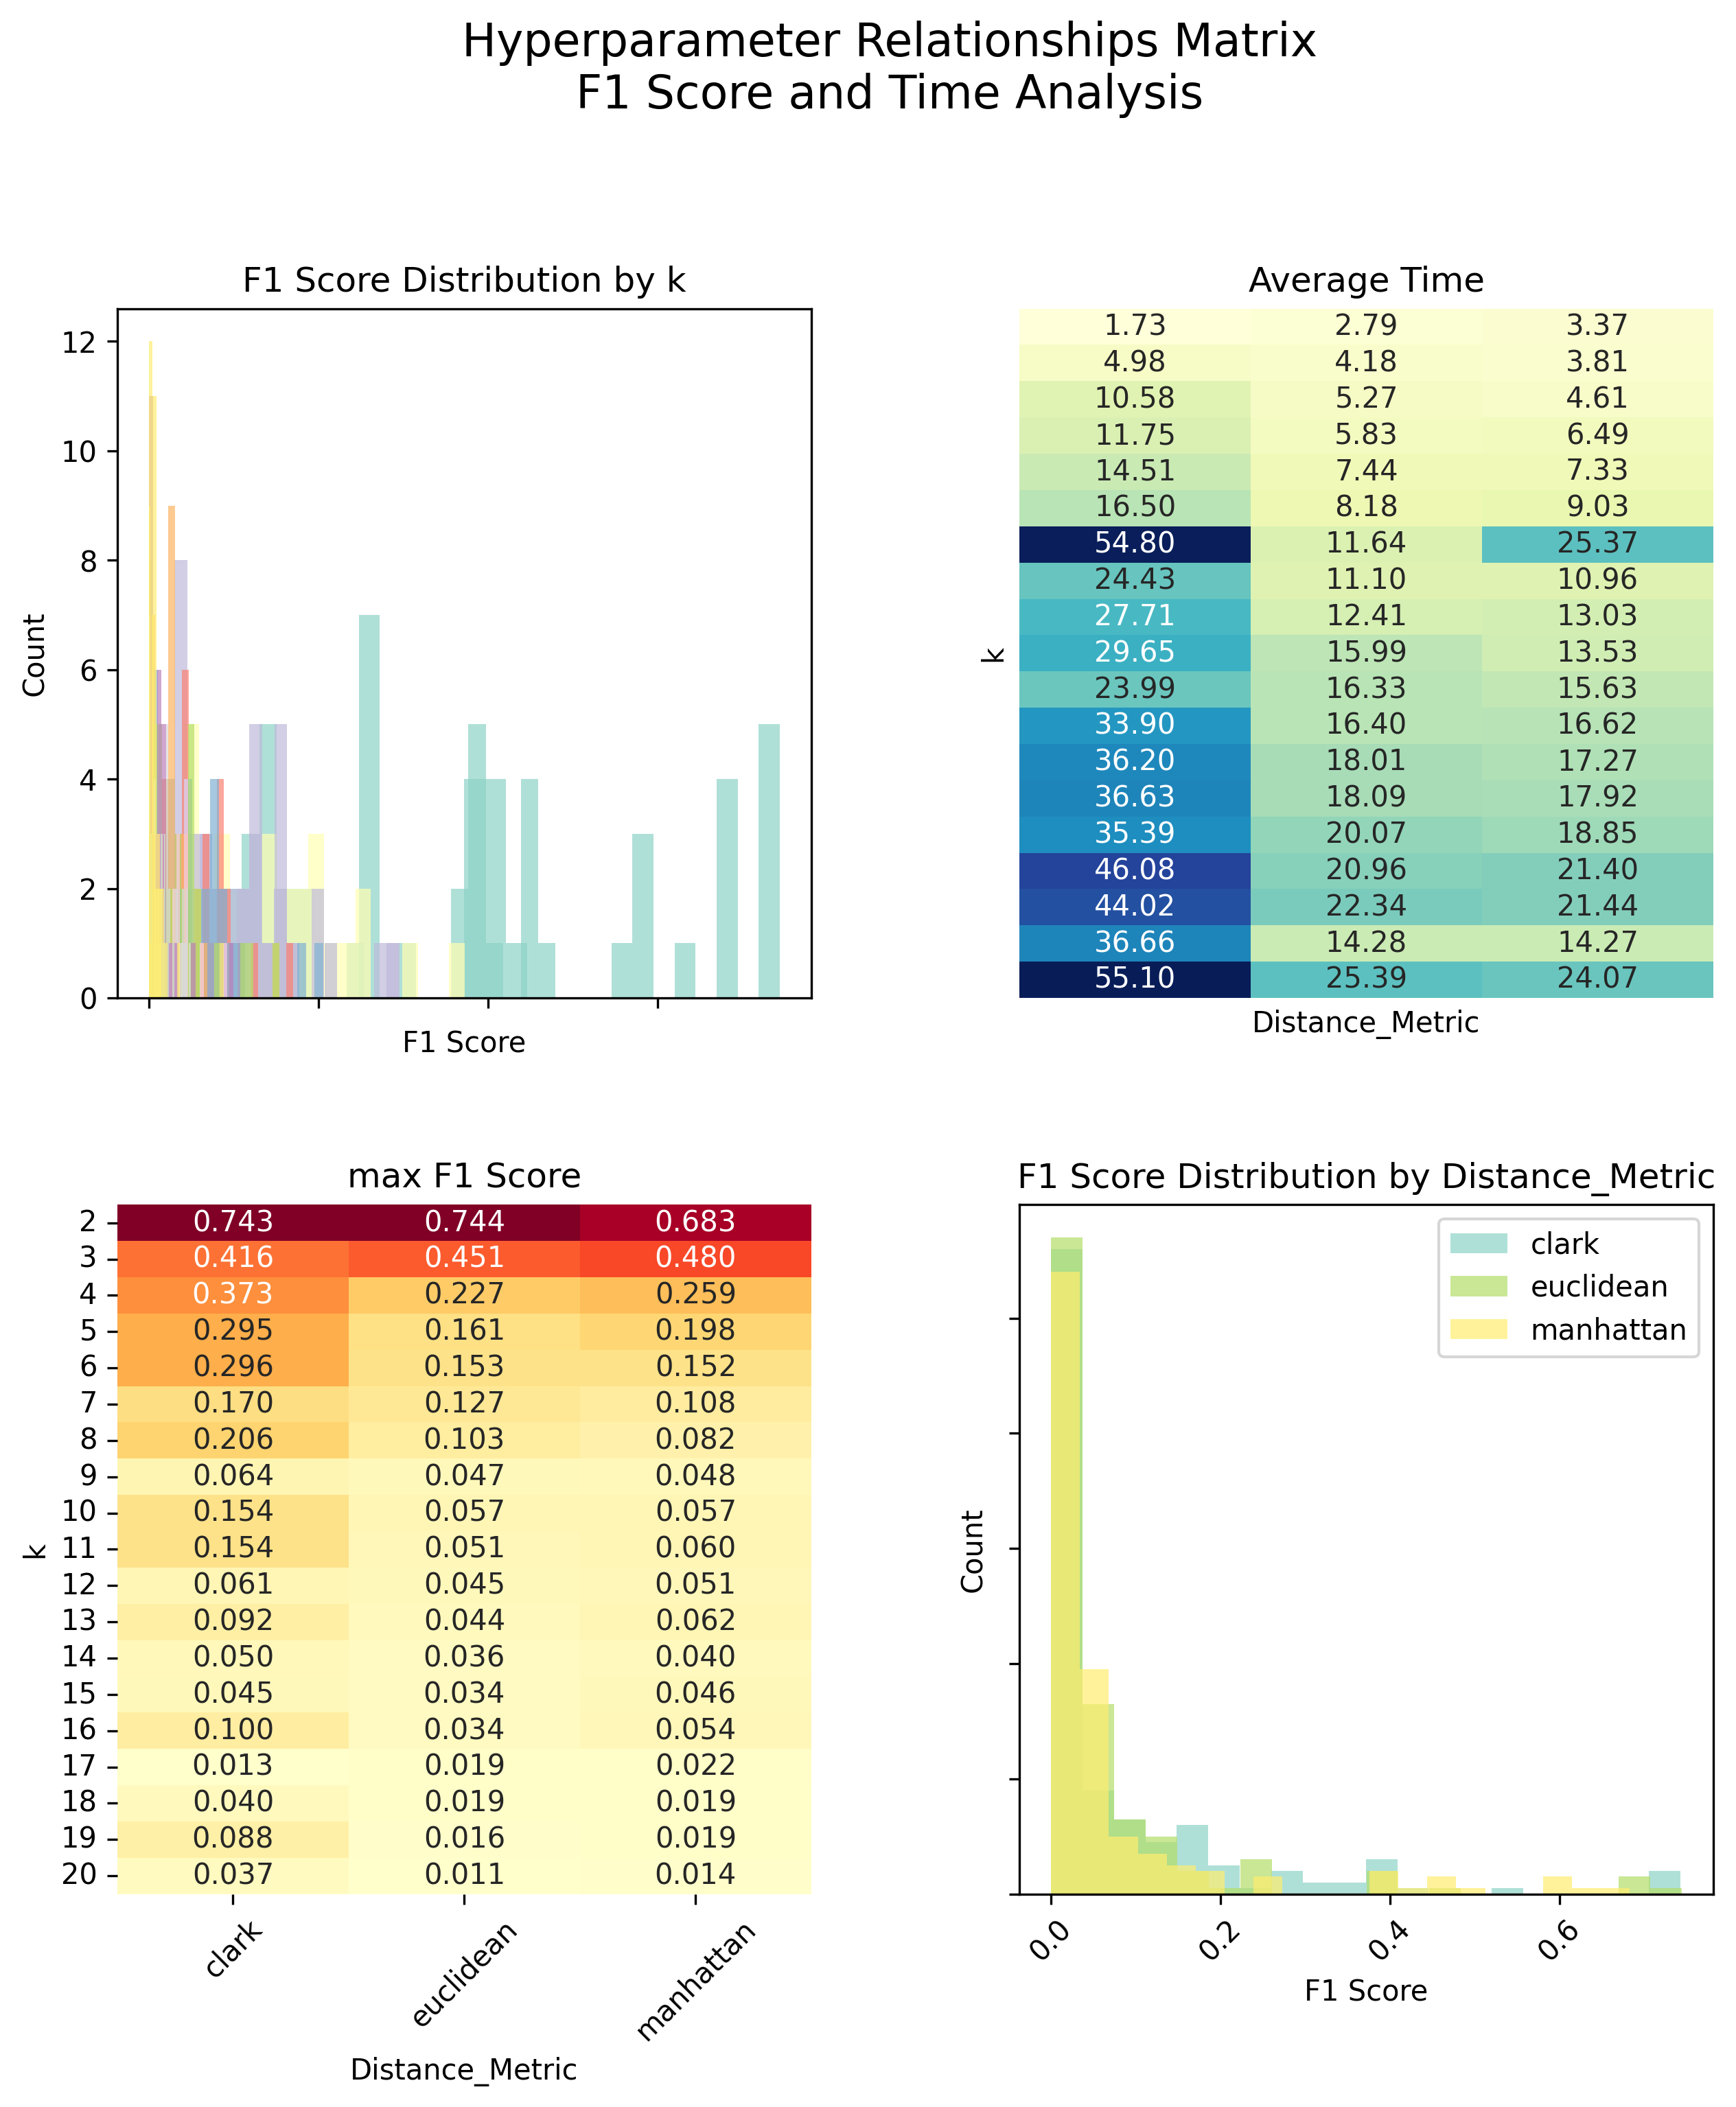
\includegraphics[width=\linewidth]{figures/mushroom_hyperparameter_pairplot_matrix.png}
        \caption{Mushroom pairplot matrix}
    \end{subfigure}
    \hfill
    \begin{subfigure}{0.49\textwidth}
        \centering
        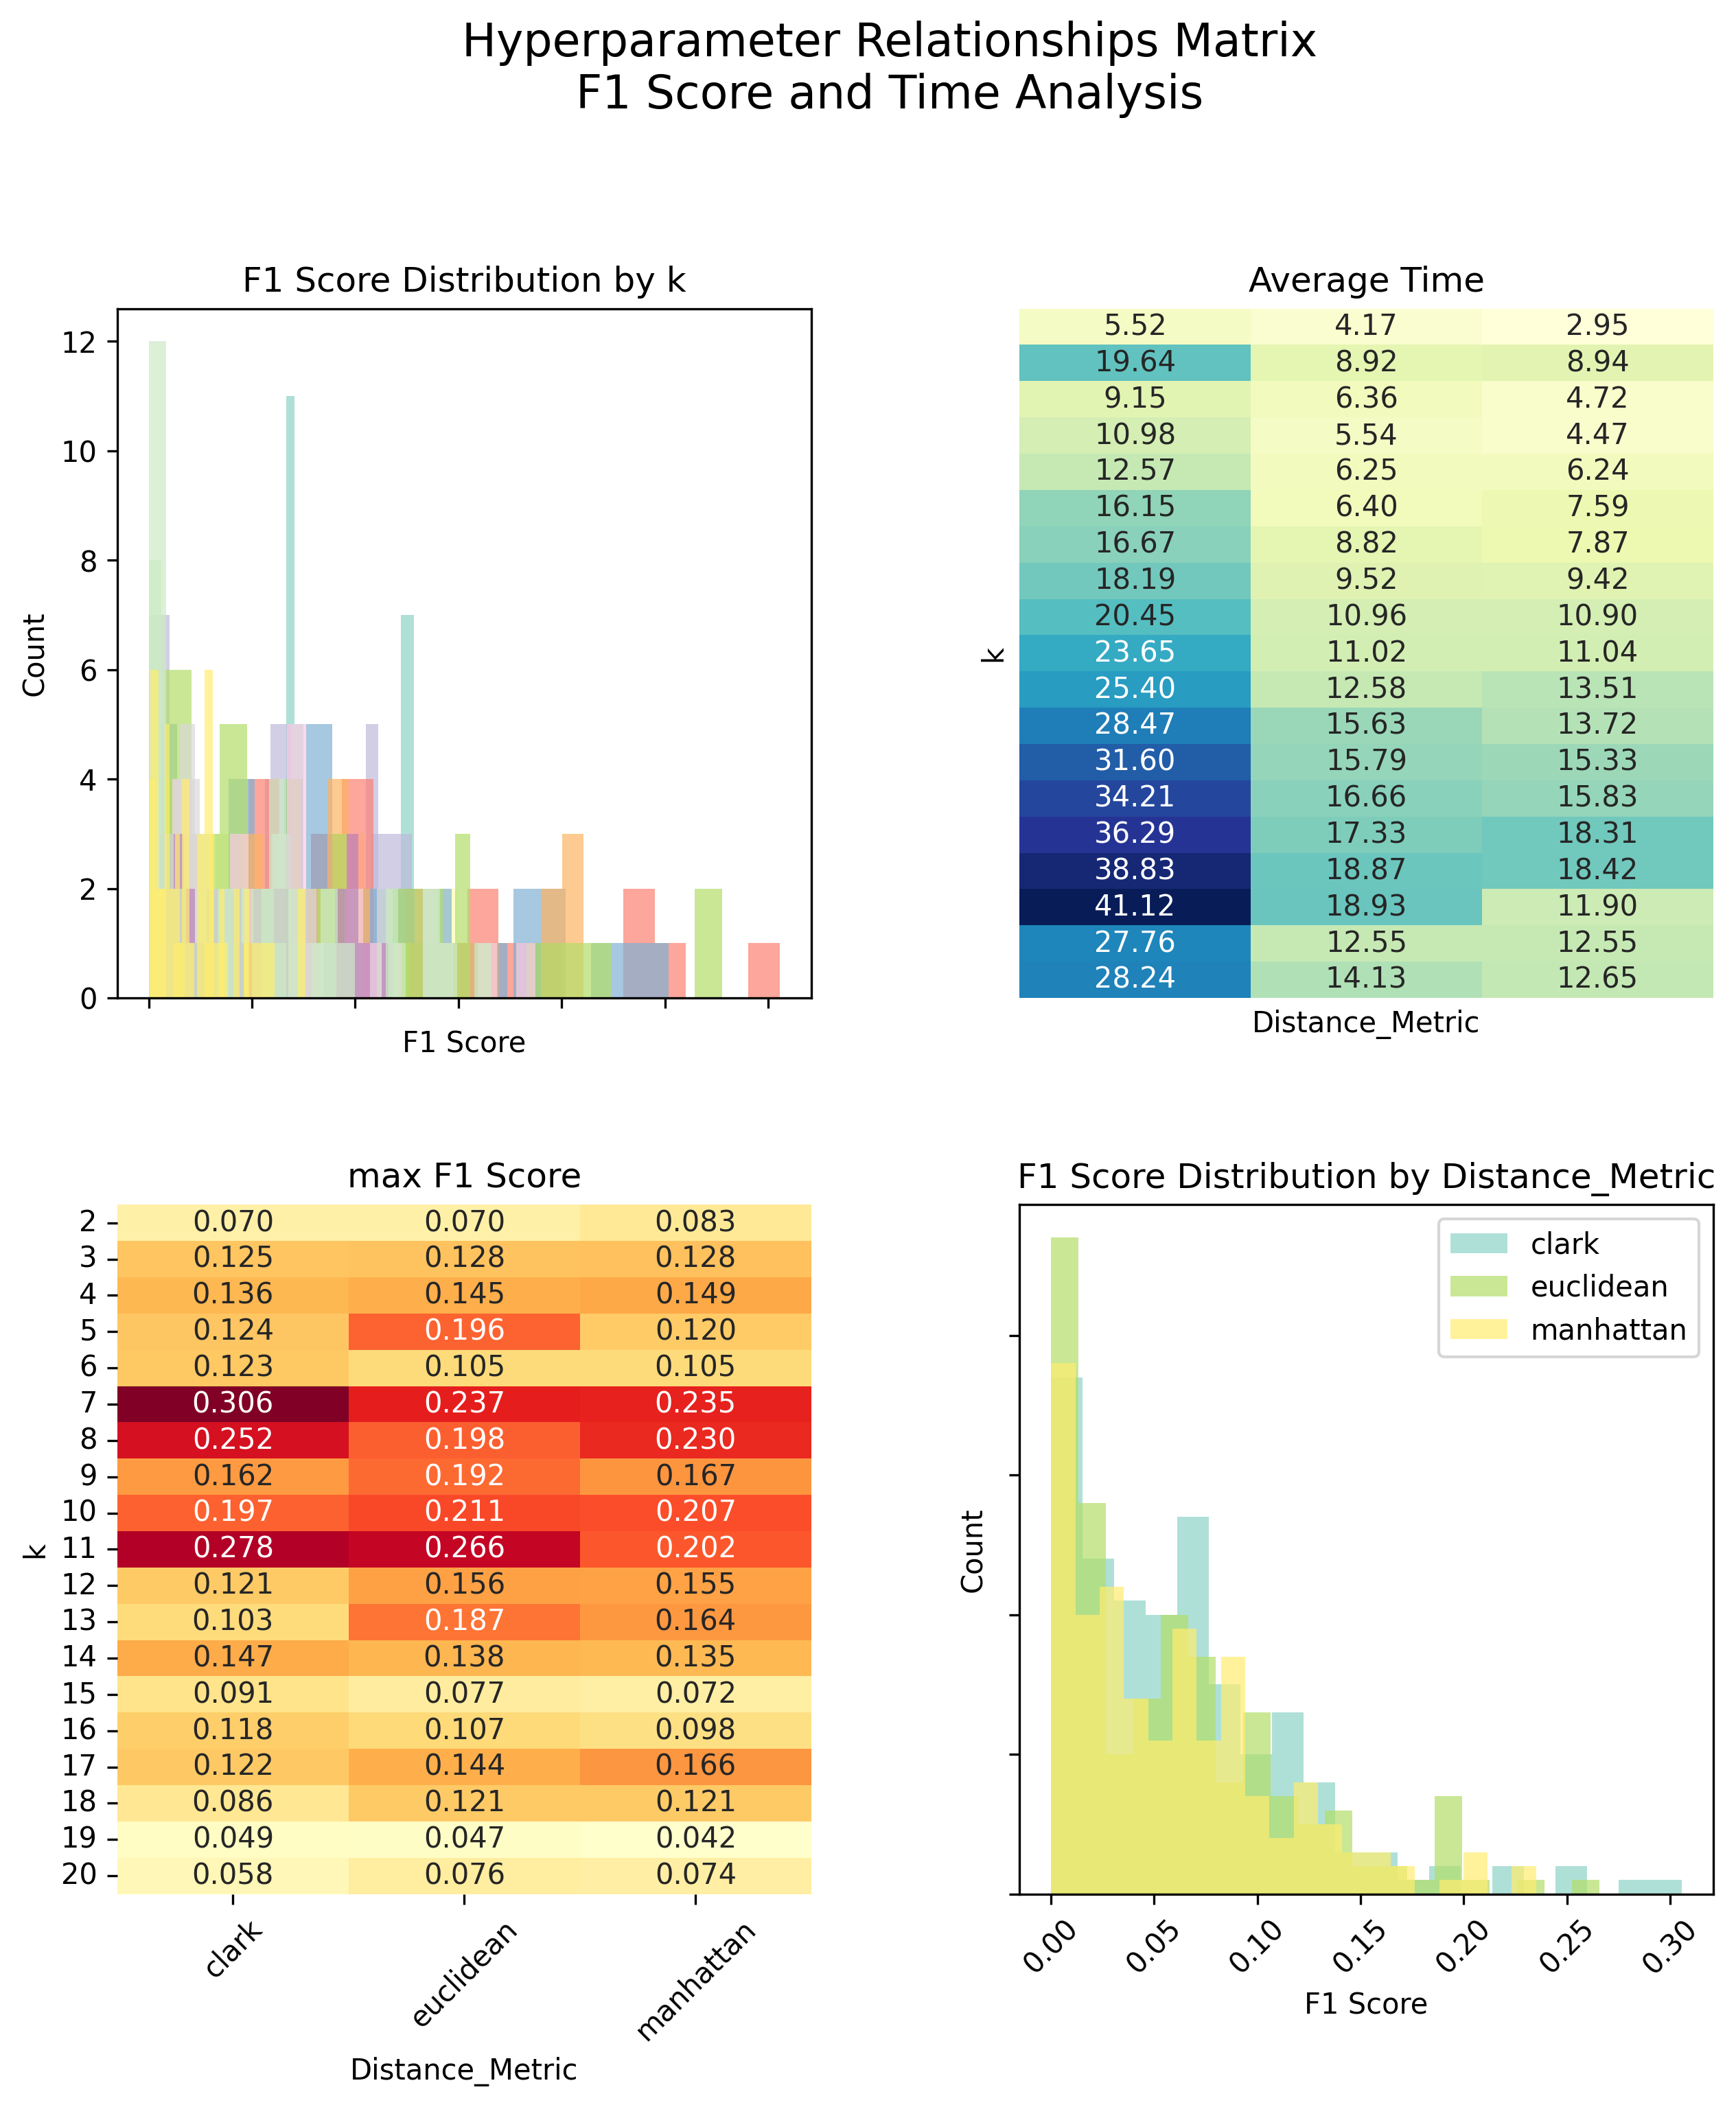
\includegraphics[width=\linewidth]{figures/penbased_hyperparameter_pairplot_matrix.png}
        \caption{Pen-based pairplot matrix}
    \end{subfigure}
    \caption{Hyperparameter pairplot matrices based on F1 Score and Time}
    \label{fig:pairplot}
\end{figure}

\subsubsection{Statistical Analysis}
For the statistical analysis, we have first performed Friedman tests to determine if there are significant differences in each of the metrics for the different possible values of each hyperparameter. 


\subsection{Global K-Means}
Out of the proposed improvements to the K-Means algorithm, the first we chose to implement was the \textbf{Global K-Means} algorithm \cite{Likas2003}, which focuses on following a deterministic and systematic approach to ``optimal'' centroid initialization and cluster formation. Additionally, we have also implemented the improvements to the Global K-Means algorithm itself, proposed in the original article by Likas et al.: \textit{Fast Global K-Means}, and \textit{Initialization with k-d Trees}. By addressing the limitations of traditional K-Means, this enhanced methodology introduces novel strategies, including PCA-based data partitioning and iterative error-reduction mechanisms, to improve both accuracy and computational efficiency.

This section outlines the hyperparameter configurations and clustering methodology adopted for the Global K-Means algorithm, which was implemented in the \texttt{GlobalKMeansAlgorithm} class.

\subsubsection{Hyperparameters}
We consider the same hyperparameters as for the standard K-Means algorithm (Section \ref{sec:kmeans}), except for 2 significant modifications:
\begin{enumerate}
    \item \textbf{Initial Centroids:}
    \begin{itemize}
        \item Global K-Means no longer accepts a collection of initial centroids as a hyperparameter, since the goal of this algorithm is rooted in the deterministic calculation of the ``best possible'' centroids, which substitutes their random initialization.
    \end{itemize}

    \item \textbf{Number of Buckets:}
    \begin{itemize}
        \item Controls initial data partitioning, by defining the number of candidate points that we will consider as possible centroids throughout the algorithm.
        \item Its default value is $2 \cdot k$, but we also test values $3 \cdot k$ and $4 \cdot k$.
    \end{itemize}
\end{enumerate}

\subsubsection{Clustering Methodology}
\begin{itemize}
    \item \textbf{Initialization with k-d Trees:}
    \begin{enumerate}
        \item Use k-d tree partitioning based on Principal Component Analysis (PCA).
        \item Recursively partition data samples into buckets.
        \item Select candidate points based on bucket centroids.
    \end{enumerate}
    \item \textbf{Fast Global K-Means Algorithm:}
    \begin{enumerate}
        \item Initialize first centroid as dataset mean.
        \item Iteratively add centroids by:
            \begin{itemize}
                \item For each $k'=2,\ldots,k$ , we already have $k'-1$ centroids.
                \item Compute guaranteed error reduction for candidate points with respect to the $k'-1$ centroids,
                \[
                b_n = \sum\limits_{j=1}^N \max\left(d_{k'-1}^j - || x_n - x_j ||^2 , 0 \right) \ ,
                \]
                where $ d_{k'-1}^j $ is the squared distance between $ x_j $ and the closest centroid among the $k'-1$ obtained so far. The pair-wise squared distances between points are precomputed at the start.
                \item Select point with maximum guaranteed error reduction.
                \item Run $k'$-means with the $k'-1$ centroids plus the selected point, unitl convergence.
            \end{itemize}
        \item Repeat until $k$ clusters are formed.
    \end{enumerate}
\end{itemize}
This methodology provides a sophisticated approach to centroid initialization and clustering, leveraging PCA-based partitioning and error reduction strategies in order to achieve an improvement in consistency and speed with respect to the base K-Means algorithm.


\section*{X-Means Algorithm}

The X-Means algorithm extends the traditional K-Means clustering algorithm by addressing its main limitations:
the need to predefine the number of clusters \( K \)
and its susceptibility to local minima. This algorithm dynamically determines the optimal number of clusters \( K \) using the Bayesian Information Criterion (BIC).

\subsection*{Core Steps of X-Means Algorithm}

The algorithm alternates between two main operations until a stopping criterion is met:

\begin{enumerate}
    \item \textbf{Improve-Parameters:} Perform standard K-Means clustering to optimize the centroid locations for a fixed number of clusters.
    \item \textbf{Improve-Structure:} Dynamically decide where to split centroids to better fit the data by evaluating each potential split using BIC.
\end{enumerate}

\subsubsection*{Splitting Process}
\begin{itemize}
    \item During the Improve-Structure step, a local K-Means with \( K = 2 \) is run until convergence for each of the clusters individually (without the rest of the clusters).
    \item After convergence, the model selection criterion (BIC score) determines whether the original parent centroid or the newly created children better represent the data. Only the better-performing structure is retained.
\end{itemize}

\subsubsection*{Stopping Criteria}
The algorithm stops when the maximum allowable number of clusters \( K_{\text{max}} \) is reached, or when no further splits improve the model selection score.

\subsection*{Model Selection Using BIC}
The Bayesian Information Criterion (BIC) for a model \( M_j \) is defined as:
\[
\text{BIC}(M_j) = L_j(D) - \frac{p_j}{2} \log R,
\]
where:
\begin{itemize}
    \item \( L_j(D) \): Log-likelihood of the data \( D \) under model \( M_j \),
    \item \( p_j \): Number of free parameters in \( M_j \),
    \item \( R \): Total number of data points.
\end{itemize}
The BIC score is calculated globally to select the best model across all iterations and locally to decide the viability of centroid splits.



\subsection{Fuzzy C-Means}

We have tested 432 different configurations of the Fuzzy C-Means (FCM) algorithm on each dataset by using the fuzziness parameter \( m \) (with values from 1.5 to 4.0) and varying the number of clusters ( n\_clusters) between the following values:

\begin{itemize}
  \item Pen-based: 6, 8, 9, 10
  \item Mushroom and Hepatitis: 2, 3, 4, 5
\end{itemize}


The following parameters were also varied:


\begin{itemize}
  \item \( \text{max\_iter} \): 100, 300, 500
  \item \( \text{error} \): 1e-1, 1e-4, 1e-5
  \item \( \rho \): 0.5, 0.7, 0.9
\end{itemize}


For each configuration, we ran the algorithm 10 times to mitigate the effects of initialization randomness, resulting in a total of 4320 runs of the FCM algorithm per dataset. From the evaluation metrics extracted in these runs, we analyze the impact of the key hyperparameters and derive insights through statistical analysis.

We decided not to include \textit{max\_iter} and \textit{error tolerance} in the analysis of performance metrics, as they do not significantly affect the performance, aside from removing outliers and slightly improving execution time. To illustrate this, we include 3 heatmaps displaying execution times for each dataset, along with the distribution of ARI results for different values of \textit{max\_iter} and \textit{error tolerance} (see \textbf{Figure}\ref{fig:error-iter-fuzzy}).


\begin{figure}[H]
    \centering
    \begin{subfigure}{0.32\textwidth}
        \centering
        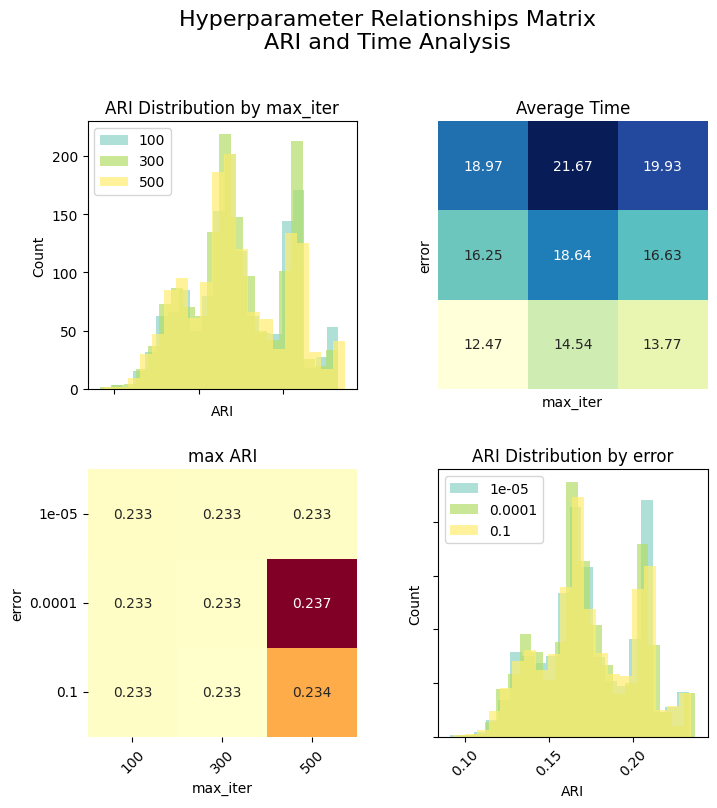
\includegraphics[width=\linewidth]{figures/FuzzyCMeans/penBased_error_iter_pairplot.png}
        \caption{Pen-based dataset.}
    \end{subfigure}
    \begin{subfigure}{0.32\textwidth}
        \centering
        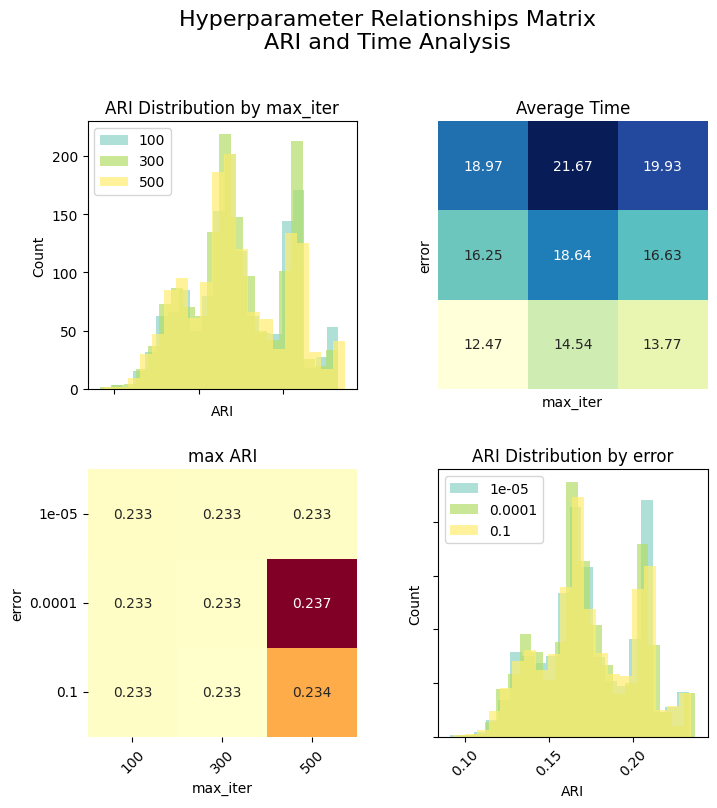
\includegraphics[width=\linewidth]{figures/FuzzyCMeans/mushroom_error_iter_pairplot.png}
        \caption{Mushroom dataset.}
    \end{subfigure}
    \begin{subfigure}{0.32\textwidth}
        \centering
        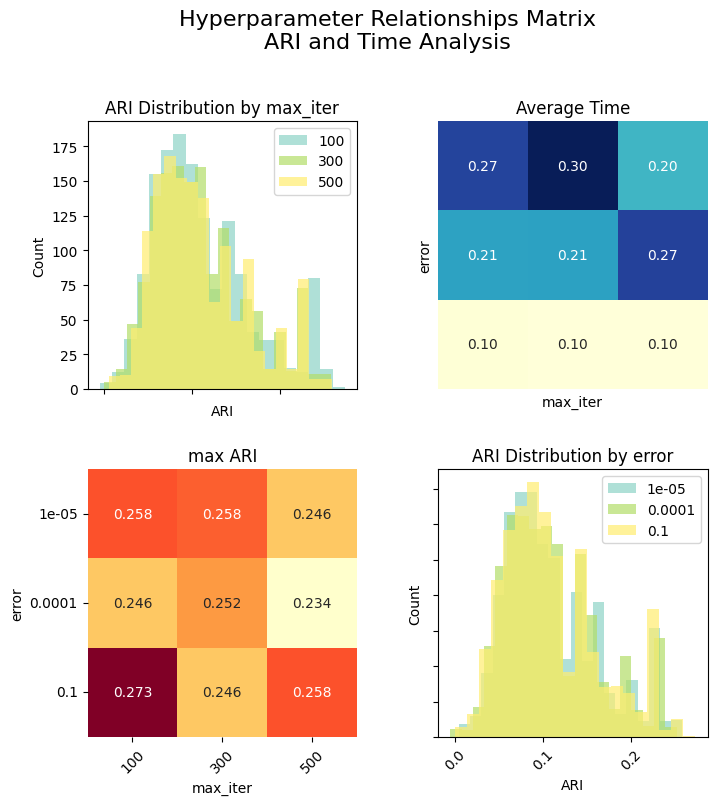
\includegraphics[width=\linewidth]{figures/FuzzyCMeans/hepatitis_error_iter_pairplot}
        \caption{Hepatitis dataset.}
    \end{subfigure}
    \caption{Heatmaps illustrating execution times for each dataset, showcasing performance across different configurations.}
    \label{fig:error-iter-fuzzy}
\end{figure}


\subsubsection{Preliminary Study}

We first explored preliminary patterns in the measured metrics and the influence of hyperparameters on clustering performance.


\textbf{Figure} \ref{fig:metrics_corr_fuzzy} illustrates the relationships between the various metrics for the FCM algorithm. This matrix plot highlights the correlations between metrics (lower triangle), histogram distributions (diagonal), and scatterplots of metric values (upper triangle). A notable observation is the interaction between the fuzziness parameter and metrics like Silhouette and DBI. For instance, while lower fuzziness (mm) often improves silhouette scores due to sharper cluster boundaries, it can lead to higher DBI values, which might indicate a trade-off between cluster compactness and interpretability. Similar trends are observed across all datasets, though the degree of correlation varies.


\begin{figure}[H]
	\centering
	\begin{subfigure}{0.32\textwidth}
		\centering
		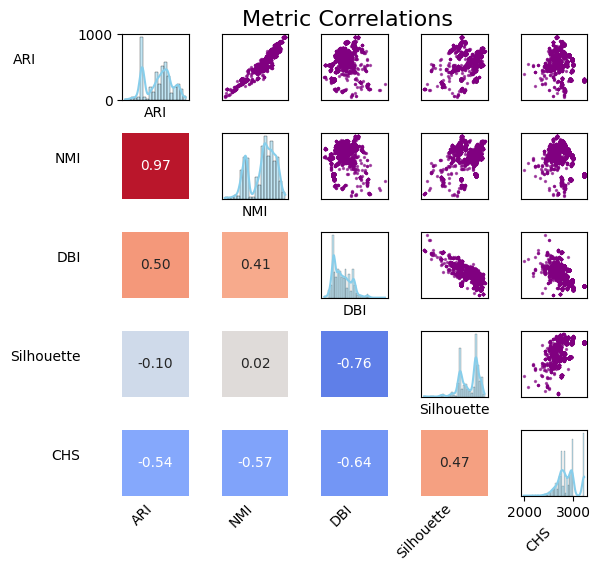
\includegraphics[width=\linewidth]{figures/FuzzyCMeans/penBased_metrics_correlations_matrix.png}
		\caption{Pen-based dataset.}
	\end{subfigure}
	\begin{subfigure}{0.32\textwidth}
		\centering
		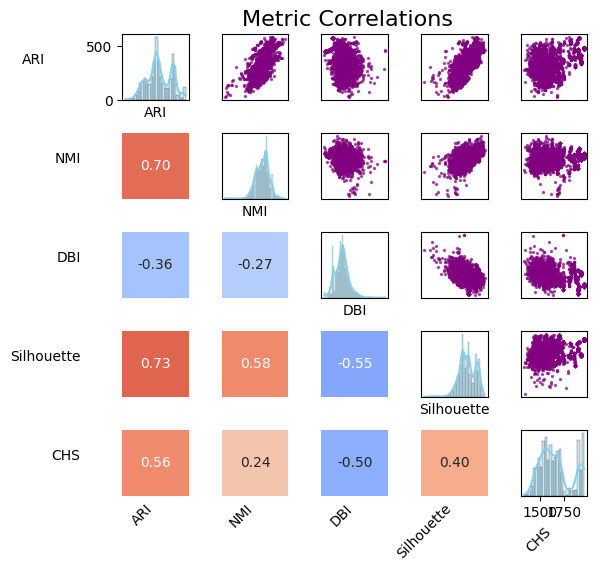
\includegraphics[width=\linewidth]{figures/FuzzyCMeans/mushroom_metrics_correlations_matrix.png}
		\caption{Mushroom dataset.}
	\end{subfigure}
	\begin{subfigure}{0.32\textwidth}
		\centering
		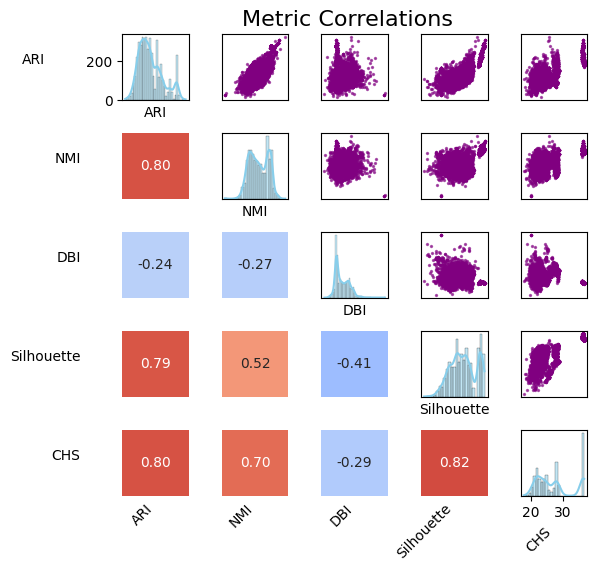
\includegraphics[width=\linewidth]{figures/FuzzyCMeans/hepatitis_metrics_correlations_matrix.png}
		\caption{Hepatitis dataset.}
	\end{subfigure}
	\caption{Metrics correlation acrross the three datasets.}
	\label{fig:metrics_corr_fuzzy}
\end{figure}


Additionally, Figure \ref{fig:pairplot_fuzzy} shows hyperparameter pairwise relationships, particularly the impact of fuzziness $m$ and number of clusters n\_clusters on clustering quality and execution time. Across datasets, higher fuzziness values consistently resulted in more computationally expensive runs, likely due to the increased complexity of assigning membership values. Interestingly, for datasets like Pen-based (10 classes), high cluster counts (e.g., n\_clusters$=10$) aligned closely with ground truth and yielded better metrics, such as ARI and NMI. Conversely, for Mushroom (2 classes), smaller values of n\_clusters and lower fuzziness performed better.


\begin{figure}[H]
\centering
\begin{subfigure}{0.49\textwidth}
\centering
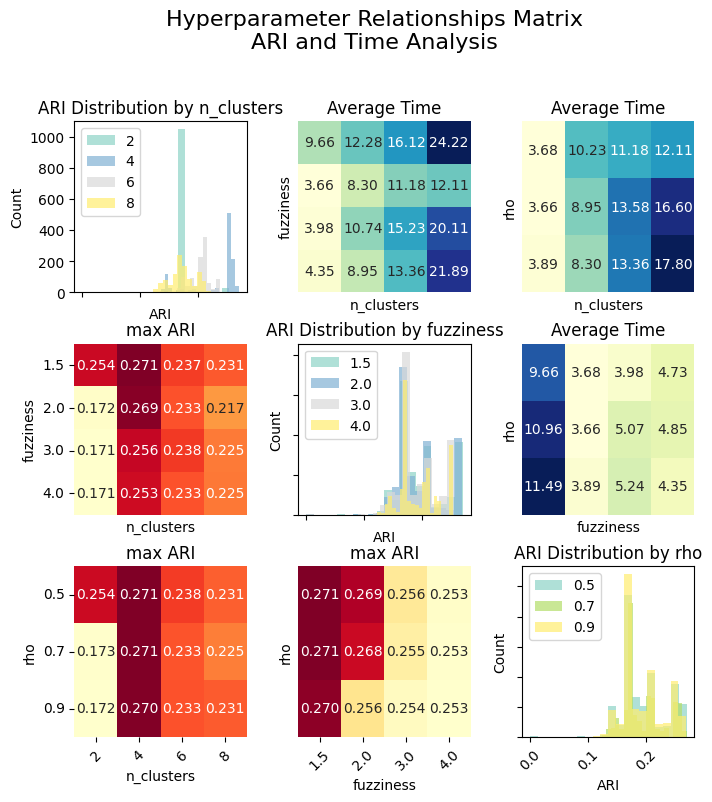
\includegraphics[width=\linewidth]{figures/FuzzyCMeans/mushroom_hyperparameter_pairplot_matrix.png}
\caption{Mushroom pairplot matrix for FCM}
\end{subfigure}
\hfill
\begin{subfigure}{0.49\textwidth}
\centering
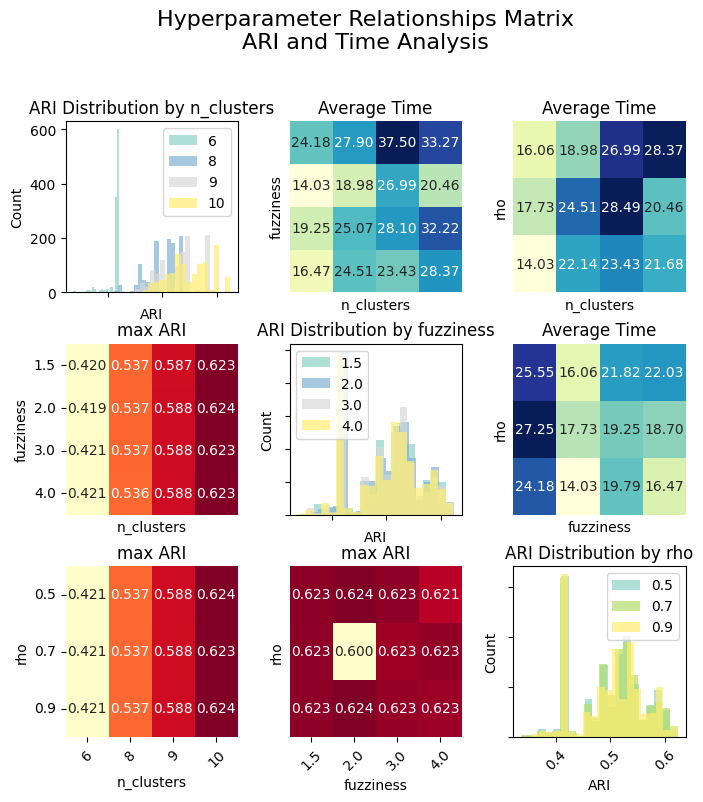
\includegraphics[width=\linewidth]{figures/FuzzyCMeans/penBased_hyperparameter_pairplot_matrix.png}
\caption{Pen-based pairplot matrix for FCM}
\end{subfigure}
\caption{Hyperparameter pairplot matrices based on clustering metrics and execution time for FCM}
\label{fig:pairplot_fuzzy}
\end{figure}



\subsubsection{Fuzziness Parameter (m):}

\begin{figure}[H]
	\centering
	\begin{subfigure}{0.32\textwidth}
		\centering
		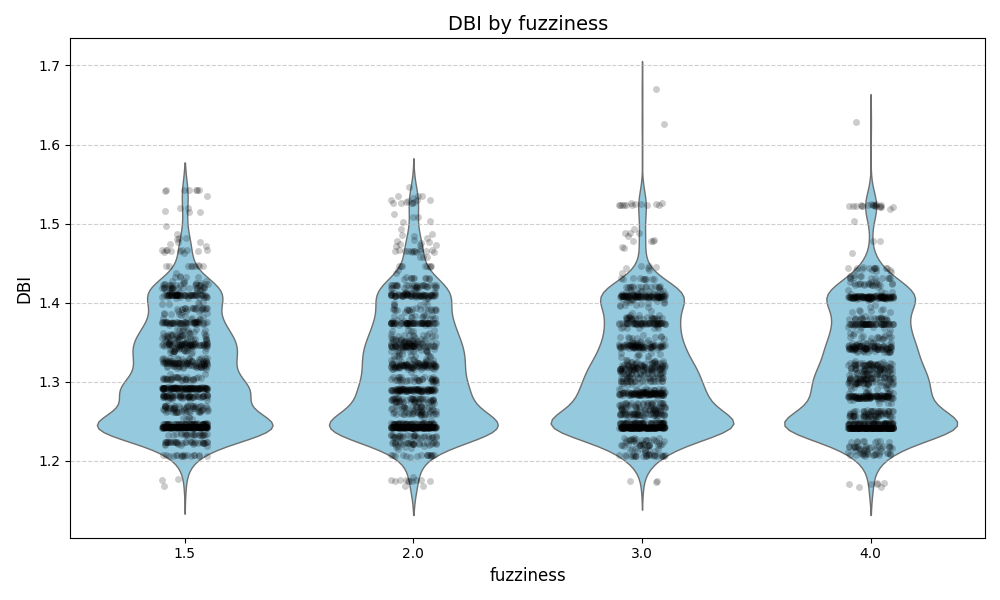
\includegraphics[width=\linewidth]{figures/FuzzyCMeans/penBased_violin_fuzziness_vs_DBI}
		\caption{Pen-based dataset.}
	\end{subfigure}
	\begin{subfigure}{0.32\textwidth}
		\centering
		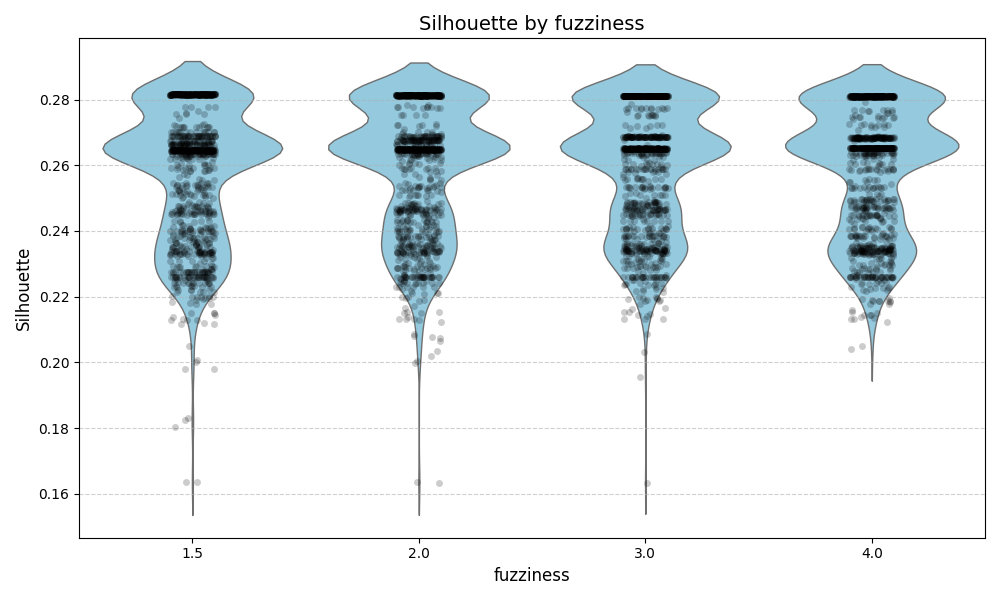
\includegraphics[width=\linewidth]{figures/FuzzyCMeans/mushroom_violin_fuzziness_vs_Silhouette}
		\caption{Mushroom dataset.}
	\end{subfigure}
	\begin{subfigure}{0.32\textwidth}
		\centering
		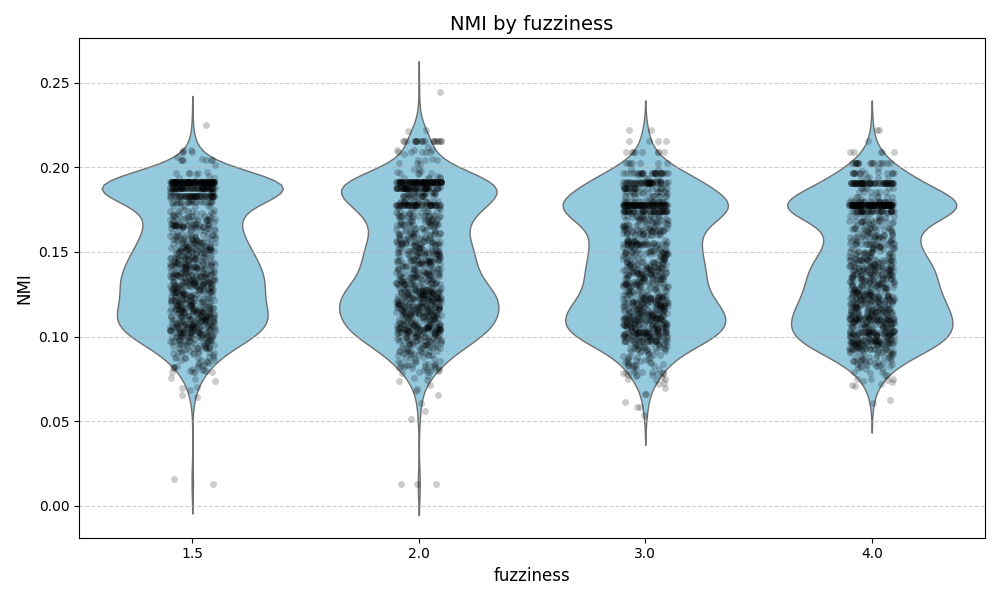
\includegraphics[width=\linewidth]{figures/FuzzyCMeans/hepatitis_violin_fuzziness_vs_NMI}
		\caption{Hepatitis dataset.}
	\end{subfigure}
	\caption{Metrics correlation acrross the three datasets.}
	\label{fig:metrics_corr_fuzzy}
\end{figure}



\begin{comment}
\subsubsection*{Number of Clusters (n\_clusters):}

\begin{enumerate}

\item Hepatitis: Lower cluster counts (e.g., n_clusters=2n\_clusters = 2) showed better ARI and Silhouette scores, aligning with the dataset's two-class structure.

\item Mushroom: Metrics like CHS favored smaller cluster counts, with n_clusters∈[2,4]n\_clusters \in [2, 4] achieving the best results. Silhouette scores corroborated these findings.

\item Pen-based: Higher cluster counts (n_clusters=10n\_clusters = 10) aligned with the dataset's class structure and yielded optimal ARI and NMI. Lower counts led to poor clustering quality, while overly high values showed diminishing returns.

\end{enumerate}

These findings confirm the sensitivity of FCM to both hyperparameters and its suitability for datasets with well-defined class structures.



\subsection*{Highlights from Tables}

\begin{itemize}

\item Pen-based Dataset: Optimal ARI (0.6242) and NMI (0.7073) achieved with n_clusters=10n\_clusters = 10 and m=2.0m = 2.0, reflecting its 10-class nature.

\item Mushroom Dataset: CHS (1962.91) supports n_clusters=6n\_clusters = 6 and m=1.5m = 1.5, showcasing the importance of small cluster counts in this two-class dataset.

\item Hepatitis Dataset: Lower n_clustersn\_clusters and fuzziness values provide better interpretability, with the highest ARI (0.1389) for m=1.5m = 1.5.

\end{itemize}

This adaptation integrates Fuzzy C-Means characteristics while maintaining your original narrative structure.
\end{comment}


\section{Conclusion}
This work explored the application of \textbf{clustering algorithms}—\textbf{K-Means}, \textbf{Global K-Means}, \textbf{X-Means} \textbf{Optics}, \textbf{Spectral Clustering}, and \textbf{Fuzzy C-Means}—across diverse datasets: \textbf{Hepatitis}, \textbf{Mushroom}, and \textbf{Pen-based}. The study revealed that clustering performance depends strongly on the \textbf{algorithm choice}, \textbf{hyperparameter configurations}, and \textbf{dataset characteristics}. 

Through this process, we learned that:
\begin{itemize}
	\item The \textbf{nature of the data} (e.g., density, dimensionality, and class distribution) significantly influences clustering quality and appropriate parameter selection.
	\item Careful \textbf{evaluation using multiple metrics} (ARI, NMI, DBI, Silhouette, and CHS) provides a more balanced view of algorithm performance, avoiding over-reliance on any single measure.
	\item Dimensionality reduction techniques, such as \textbf{PCA} and \textbf{UMAP}, play a crucial role not only in visualization but also in understanding \textbf{hidden structures} within the data.
	\item Robust clustering outcomes often require a \textbf{systematic approach to hyperparameter tuning}, tailored to the dataset's specific properties.
\end{itemize}

The main lesson learned is that no single clustering method is universally optimal. Instead, the choice of method and configuration must be \textbf{data-driven} and guided by domain knowledge. Future work could explore integrating clustering algorithms with ensemble methods or hybrid approaches to further enhance performance across complex datasets.

In summary, this study highlights the importance of \textbf{methodological rigor} and \textbf{data-aware experimentation} when applying clustering techniques. The lessons learned can provide practical guidelines for adapting these methods to real-world problems.
\newpage

\bibliographystyle{plain}
\bibliography{references}

\end{document}

